\chapter{Basic Theory of Pseudo Differential Operators}\label{chap4}

\section{Representation of Pseudo differential Operators}\label{chap4:sec1}

Let\pageoriginale $L = \sum \limits_{|\alpha | \le k} a_\alpha (x)D^\alpha $ be a
partial differential operator with $C^\infty$ coefficients on
$\Omega$. Using the Fourier transform, we can write 
\begin{align*}
(Lu)(x) & = \sum_{|\alpha| \le k}  a_\alpha (x) \int e^{2 \pi
    ix.\xi}\hat{u}(\xi)\xi^\alpha d \xi\\ 
  & = \int e^{2 \pi ix. \xi}p(x, \xi)\hat{u}(\xi)d \xi
\end{align*}
where $p(x, \xi)= \sum\limits_{|\alpha| \le k}  a_\alpha (x)
\xi^\alpha$. This representation suggests that $p(x,\xi)$ can be
replaced by more general functions. So, we make the following
definition. 

\begin{defi}\label{chap4:sec1:def4.1}
  For an open set $\Omega \subset \mathbb{R}^n$ and a real number $m$ we
  define $S^m(\Omega)$, the class of symbols of order $m$ on $\Omega$,
  by 
  $$
  S^m(\Omega)= \{p \epsilon C^\infty(\Omega \times \mathbb{R}^n) :
  \forall \alpha, \beta, V \Omega' \subset \Omega, ~c=c_{\alpha \beta
    \Omega'} 
  $$
  such that  $\sup_{x \epsilon \Omega'}  |D^\beta_x D^\alpha_\xi p(x,
  \xi)| \le c (1+| \xi |)^{m-|\alpha|}\}$. 
\end{defi}

We note that $S^m(\Omega) \subset S^m$ whenever  $m < m'$, and we set
$S^{- \infty}(\Omega)= \bigcap \limits_{m \epsilon \mathbb{R}}
S^m(\Omega)$.

\medskip 
\noindent \textbf{Examples}
  \begin{enumerate}[\rm (i)]
  \item Let $p(x,\xi)=\sum\limits_{|\alpha|\le k} a_\alpha(x)\xi^\alpha
  $ with $a_\alpha \epsilon C^\infty (\Omega)$. Then $p \epsilon
  S^k (\Omega)$. 
\item Let\pageoriginale $p(x,\xi) = \sum\limits^{N}_{j=1} a_j (x) f_j(\xi)$ where
  $a_f \epsilon  C^\infty (\Omega)$ and $f_j \epsilon C^\infty
  (\mathbb{R}^n)$ is homogeneous of degree $m_j$ large $\xi $ : that
  is, 
  $$
  f_i(r \xi)=r^{m_j} f_j(\xi) \text{ for } |\xi| \ge c, r \ge 1.
  $$

  In this case, $p \epsilon S^m(\Omega)$, where $m= \max\limits_{1 \le j \le 
    N}\{m_j\}$.  
\item Let $p(x,\xi) = (1+| \xi |^2)^{s/2}$. This $p$ belongs to
  $S^s(\mathbb{R}^n)$. 
\item Let $p(x,\xi)= \phi(\xi) \sin \log |\xi|$ with $\phi \epsilon
  C^\infty,  \phi =0$ near the origin and $\phi =1$ when $|\xi| \ge
  1$. Then $p \epsilon S^o (\mathbb{R}^n)$. 
\end{enumerate}

\setcounter{rem}{1}
\begin{rem} \label{chap4:sec1:rem4.2}
  We observe that when $ p \epsilon S^m (\Omega),  D^\beta_x
  D^\alpha_\xi  p \epsilon S^{m-|\alpha|}(\Omega)$. 
\end{rem}

Further, if $p \epsilon S^{m_1}(\Omega)$ and $q \epsilon
S^{m_2}(\Omega)$,then $p+q \epsilon S^m(\Omega)$, where $m=\max
\{m_1,m_2\}$ and $pq \epsilon S^{m_1 +m_2}(\Omega)$. 

\begin{rem}\label{chap4:sec1:rem4.3}
  Our symbol classes $S^m(\Omega)$ are special cases of Hormander's
  classes $S^m_{\rho, \delta}(\Omega)$. Namely, for $0 \le \delta \le
  \rho \le 1$, and $m \epsilon \mathbb{R}$, 
  $$
  \displaylines{\hfill
  S^m_{\rho, \delta}(\Omega)=\{p \epsilon C^\infty (\Omega \times
  \mathbb{R}^n) : \forall \alpha, \beta, V \Omega' \Subset \Omega,
  c=c_{\alpha \beta \Omega'}\hfill \cr 
  \text{such that} \hfill \sup_{x \epsilon \Omega'}| D^\beta_x D^\alpha_\xi p (x,
  \xi)| \le c (1+|\xi|)^{m-\rho | \alpha |+\delta |\beta|}\}.\hfill} 
  $$
  In this terminology, $S^m (\Omega)= S^m_{1,0}(\Omega)$.
\end{rem}

\setcounter{defi}{3}
\begin{defi}\label{chap4:sec1:def4.4}
  For $p \epsilon S^m (\Omega)$, we define the operator $p(x.D)$ on
  the domain $C^\infty_o (\Omega)$ by  
  $$
  p(x,D)\, u(x)= \int e^{2 \pi i x. \xi }p(x,\xi)\,\hat{u}(\xi)d \xi, u
  \epsilon C^\infty_o(\Omega). 
  $$
\end{defi}

(Sometimes, we shall denote $p(x,D)$ by $p$). Operators of the form
$p(x,D)$\pageoriginale with $p \epsilon S^m (\Omega)$ are called \textit {pseudo
  differential operators of order} $m$ on $\Omega$. 

The set of all pseudo differential operators of order $m$ on $\Omega$
will denoted by $\Psi^m (\Omega)$. For brevity, we will sometimes
write $``\Psi D O''$ instead of  ``pseudo differential operators''. 

The next theorem states that $p(x,D)$ is a continuous linear map of
$C^\infty_o (\Omega)$ into $C^{\infty} (\Omega$ which extends to
$E'(\Omega)$. For the proof, we need a result which depends on  

\setcounter{lem}{4}
\begin{lem} \label{chap4:sec1:lem4.5}
  Let $p \epsilon S^m (\Omega)$ and $\phi \epsilon C^\infty_o
  (\Omega)$. Then, for each positive integer $N$, there exists $c_N >
  0$ such that for all $\xi, \eta $ in $\mathbb{R}^n$, 
  $$
  |\int e^{2 \pi i x.\eta}p(x,\xi) \phi (x) dx|\le c_N (1+|\xi|)^m (1+|\eta |)^{-N}.
  $$
\end{lem}

\begin{proof}
  For any $\xi$ and $\eta$ in $\mathbb{R}^n$,

  $| \eta^\alpha \int e^{2 \pi i x.\eta}p(x,\xi) \phi (x) dx |$
  $$
  = | \int D^\alpha_x e^{2 \pi i x.\eta}p(x,\xi) \phi (x) dx |.
  $$
\end{proof}

Integrating by parts, we have
\begin{align*}
| \eta^\alpha \int e^{2 \pi i x.\xi}p(x,\xi) \phi (x) dx |
  = &~ | \int e^{2 \pi i x.\eta} D^\alpha_x (p(x,\xi) \phi (x)) dx |\\
\le &~ C_\alpha (1+|\xi|)^m \text{ for all } \alpha.
\end{align*}

Therefore
$$
\sum_{| \alpha| \le N}| \eta^\alpha \int e^{2 \pi i
  x.\eta}p(x,\xi)\phi(x)dx|\le c'_N(1+|\xi|)^m \text{ for all } N. 
$$

Since\pageoriginale $(1+| \eta)^N \le c \sum\limits_{| \alpha| \le N}| \eta^\alpha
|$, the required result follows. 

\setcounter{coro}{5}
\begin{coro} \label{chap4:sec1:coro4.6}
If $p \epsilon S^m (\Omega)$ and $\phi \epsilon C^\infty_o
  (\Omega)$, then the function 
$$
g(\xi)= \int e^{2 \pi ix. \xi} p(x,\xi)\phi (x)dx
$$
is rapidly decreasing as $\xi$ tends to $\infty$.
\end{coro}

\begin{proof}
  Set $\xi = \eta$ in the lemma.
\end{proof}

\setcounter{thm}{6}
\begin{thm} \label{chap4:sec1:thm4.7}
  If $p \epsilon S^m(\Omega)$, then $p(x,D)$ is a continuous
    linear map of $C^\infty _o(\Omega)$ into $C^\infty (\Omega)$ which
    can be extended as a linear map from $E'(\Omega)$ into
    $D'(\Omega)$. 
\end{thm}

\begin{proof}
  For $u \epsilon C^\infty_o (\Omega)$,
  $$
  p(x,D)u(x)= \int e^{2 \pi ix.\xi} p(x,\xi)\hat{u}(\xi)d \xi.
  $$

  The integral converges absolutely and uniformly on compact sets, as do
  the integrals 
  $$
  \int D^\alpha_x(e^{2 \pi ix.\xi} p(x,\xi)\,\hat{u}(\xi)d \xi \text{ for
    all }\alpha, 
  $$
  since $p \epsilon S^m$ and $\hat{u} \epsilon \mathcal{S}$.
\end{proof}
  This proves that $p(x, D)u \epsilon C^\infty (\Omega)$, and
  continuity of $p(x, D)$ from $C^\infty_o (\Omega)$ to $C^\infty
  (\Omega)$ is an easy exercise.

To prove the rest of the theorem, we will make use of
Corollary \ref{chap4:sec1:coro4.6}.

For $u \epsilon E'(\Omega)$, we define $p(x,D)u$ as a functional on
$C^\infty_o(\Omega)$ as follows: 
\begin{align*}
  < p(x,D)u, \phi > & = \iint p(x,\xi) \hat{u}(\xi) e^{2 \pi ix.\xi}
  \phi(x)dx d \xi \\ 
  & = \int g(\xi)\hat{u}(\xi) d\xi
\end{align*}
where\pageoriginale
$$
g(\xi)=\int e^{2 \pi ix.\xi} p(x,\xi)\phi(x)dx, \text{ for }  \phi
\epsilon C^\infty_o(\Omega). 
$$

By Corollary \ref{chap4:sec1:coro4.6}, $g(\xi)$ is rapidly decreasing, while $\hat{u}$ is
of polynomial growth; so the last integral is absolutely convergent
and the functional on $C^\infty_o$ thus defined is easily seen to be
continuous. Moreover,  if $u \epsilon C^\infty_o$, the double
integral is absolutely convergent, and by interchanging the order of
integration, we see that this definition of $p(x,D)u$ coincides with
the original one. Hence we have extended $p(x,D)$ to a map from
$E'(\Omega)$ to $\mathcal{D}(\Omega)$. 

\setcounter{rem}{7}
\begin{rem} \label{chap4:sec1:rem4.8}
  It follows easily from the above argument that $p(x,D)$ is
  sequentially from $E'(\Omega)$ to $\mathcal{D}(\Omega)$, i.e., if
  $u_k$ converges to $u$ in $E'(\Omega)$, then $p(x,D)u_k$ converges to
  $p(x,D)u$ in $\mathcal{D}'(\Omega)$. Actually, $p(x,D)$ is continuous
  from $E'(\Omega)$ to $\mathcal{D}'(\Omega)$ : this follows from the
  fact (which we shall prove later) that the transpose of a pseudo
  differential operator is again a pseudo differential operator. Thus
  $p(x,D)^t : C^\infty_o(\Omega) \to C^\infty(\Omega)$ is continuous,
  and so, by duality, $p(x,D)=(p(x,D)^t)^t : E'(\Omega) \to
  \mathcal{D}'(\Omega)$ is continuous. 
\end{rem}

\section{Distribution Kernels and the Pseudo Local Property}\label{chap4:sec2}

\setcounter{defi}{8}
\begin{defi} \label{chap4:sec2:def4.9}
  Let $T$ be an operator from $C^\infty_o(\Omega)$ to
  $C^\infty(\Omega)$. If there exists a distribution $K$ on $\Omega
  \times \Omega$ such that  
  $$
  < Tu, v > = < k, v \otimes u > \text{ for } u,v \epsilon C^\infty_o
  (\Omega),  
  $$
  we say that $K$ is the {\em distribution kernel} of the operator $T$.
\end{defi}

In this definition, $v \otimes u$ is defined by $(v \otimes u)(x,y)=v(x)u(y)$.
Formally, this definition says that.
$$
Tu(x)=\int K(x.y) u (y)dy.
$$\pageoriginale
$K$ is uniquely determined since linear combinations of functions of
the form $v \otimes u$ are dense in $C^\infty_o (\Omega \times
\Omega)$. 

If $ p \epsilon S^m(\Omega)$, it is easy to compute the
distribution kernel of $p(x,D)$. In fact, 
\begin{align*}
  < p(x,D)u,v> &= \iint p(x, \xi)\hat{u}(\xi) e^{2 \pi ix.\xi}v(x)d \xi dx\\
  &= \iint p(x, \xi) e^{2 \pi ix.\xi}(v \otimes u)^{\hat{}}_2 (x,\xi) d \xi dx
\end{align*}
where $(v \otimes u)^{\hat{}}_2 (x,\xi)$ means the Fourier transform
in the second variable. 


It follows immediately from the definition of $K$ that
\begin{align*}
  <  K,w > &= \iint e^{2 \pi ix.\xi}p(x,\xi)w^{\hat{}}_2 (x,\xi) d\xi
  dx, \forall w \epsilon C^\infty_o (\Omega \times \Omega). \\ 
  \text{ or } <K,w> &= \iiint e^{2 \pi i(x-y).\xi} p(x,\xi)w(x,y)dy~d\xi~dx.
\end{align*}

From this it is easy to see that $K(x,y)=p^v_2(x, x-y)$ where
$p^v_2(x,.)$ is the inverse Fourier transform of the tempered
distribution $p(x,.)$. In particular, this shows that $p$ is uniquely
determined by the operator $p(x,D)$. If $P \epsilon
\Psi^m(\Omega)$, we shall sometimes denote the unique $p \epsilon
S^m(\Omega)$ such that $p=p(x,D)$ by $\sigma_p$. 

The following theorem gives precise results on the kernel $K$ of
\break $p(x,D)$.

\setcounter{thm}{9}
\begin{thm} \label{chap4:sec2:thm4.10}
The distribution kernel $K$ of $p(x,D)$ with $p \epsilon
  S^m(\Omega)$ is in $C^\infty$ on $(\Omega \times \Omega) \slash
  \Delta$ where $\Delta \{(x,x): x \epsilon \Omega\}$ is the
  diagonal. More precisely, if $|\alpha |> M+n+j$ for a positive
  integer $j$, then $(x-y)^\alpha K(x,y)\epsilon C^j (\Omega \times
  \Omega)$. 
\end{thm}

\begin{proof}
For\pageoriginale $w \epsilon C^\infty_o(\Omega \times \Omega)$, let us compute
$<(x-y)^\alpha K, w >$. 
\begin{align*}
  < (x-y)^\alpha K,w > &=< K,(x-y)^\alpha w >\\
  &= \iint e^{2 \pi ix.\xi}p(x,\xi)(x+D_\xi)^\alpha w^{\hat{}}_2(x,\xi)d \xi~dx\\
  &= \iint w^{\hat{}}_2(x,\xi)(x-D_\xi)^\alpha \{ e^{2 \pi ix.\xi}p(x,\xi)\}d \xi~dx.
\end{align*}
\end{proof}

Using the Leibniz formula, it is easily seen that
$$
(x-D_\xi)^\alpha \{e^{2 \pi ix.\xi}p(x,\xi)\}= (-D_\xi)^\alpha
p(x,\xi).e^{2\pi ix.\xi} 
$$

Therefore
\begin{align*}
  <(x-y)^\alpha K,w > &= \iint w^{\hat{}}_2(x,\xi)e^{2 \pi
    ix.\xi}(-D_\xi)^\alpha p(x,\xi)d\xi~dx\\ 
  &= \iiint w(x,y)e^{2 \pi i(x-y).\xi}(-D_\xi)^\alpha p(x, \xi)dy~d\xi~dx.
\end{align*}

From the above expression, we infer that
$$
(x-y)^\alpha K(x,y)=\int e^{2 \pi i(x-y).\xi}(-D_\xi)^\alpha p(x,\xi)d \xi.
$$

Since $|(-D_\xi)^\alpha p(x,\xi)|\le c(1+|\xi|)^{m-|\alpha|}$, the
integral converges absolutely and uniformly on compact sets whenever
$m-|\alpha | < -n$.  Also we can differentiate with respect to $x$ and
$y \quad j$ times under the integral sign provided $m-|\alpha|+j<-n$
or $|\alpha|> m+n+j$. Thus, we see that $(x-y)^\alpha K \epsilon
C^j(\Omega \times \Omega)$. 

\setcounter{coro}{10}
\begin{coro}[PSEUDO LOCAL PROPERTY OF $\Psi DO$]\label{chap4:sec2:coro4.11} 
  If $P \epsilon \Psi^m$ $(\Omega)$, then, for all $u \epsilon E'(\Omega)$, sing
  $\supp$ Pu is contained in sing $\supp u$. 
\end{coro}

\begin{proof}
  Let $u \epsilon E'$ and let $V$ be an arbitrary neighbourhood of
  sing supp $u$. Take a $\phi \epsilon C^\infty _o(V)$ such that
  $\phi=1$ on sing supp $u$. Then $u=\phi u +(1- \phi) u = u_1 + u_2 ;
  u_2$ is a $C^\infty_o$ function and supp $u_1 \epsilon V$.  
\end{proof}

Therefore, $Pu = Pu_1  + Pu_2$ and $Pu_2$ is a $C^\infty$
function. Moreover, when $x_o \notin V$,\pageoriginale 
$$
Pu_1(x) = \int_V K(x,y) u_1 (y) dy
$$
is also a $C^\infty$ function in a neighbourhood of $x_o$ since
$u_1(y) = 0$ for $y$ near $x_o$. This implies that sing supp $Pu
\subset V$. Since $V$ is any neighbourhood of sing supp $u$, the
corollary is proved. 

\setcounter{coro}{11}
\begin{coro}\label{chap4:sec2:coro4.12}
  If $p \epsilon S^{- \infty}(\Omega)$, then the distribution
  kernel $K$ of $p(x,D)$ is in $C^\infty (\Omega \times \Omega)$. 
\end{coro}
\begin{proof}
  Follows from the theorem if we take $|\alpha|=0$.
\end{proof}


\begin{coro}\label{chap4:sec2:coro4.13}
  If $p \epsilon S^{-\infty}(\Omega)$, then $p(x,D)$, maps
  $E'(\Omega)$ continuously into $C^\infty(\Omega)$. 
\end{coro}
\begin{proof}
  If $u \epsilon E'(\Omega)$, in view of Corollary 4.12, it is
  easily seen that \break $p(x,D)u$ is a smooth function defined by  
  $$ 
  P(x,D)u(x) = \int K(x,y) u (y) dy = <u, K (x,.) >,
  $$
  whence the result follows.
\end{proof}

\setcounter{defi}{13}
\begin{defi} \label{chap4:sec2:def4.14}
  A smoothing operator is a linear operator $T$ which maps
  $E'(\Omega)$ continuously into $C^\infty (\Omega)$. 
  
  If $K \epsilon C^\infty (\Omega \times \Omega)$, then the operator
  $T$ defined by  
  $$
  (Tf)(x)=< K(x,.), f> =\int K(x,y)f(y)dy
  $$
  is a smoothing operator.  Conversely,  every smoothing operator $T$
  can be given in the above form with $K(x,y)=(T \delta_y)(x)$. 
\end{defi}

As we have already remarked if $p \epsilon S^{-\infty}$, then the
corresponding $\Psi DO$ is smoothing. However, not every smoothing
operator is a $\Psi DO$. For example, we have 

\setcounter{prop}{14}
\begin{prop}\label{chap4:sec2:prop4.15}
  Suppose\pageoriginale $p(x,.)$ is a $C^\infty$ function of $x$ with values in
  $E'$. Then $p(x,D)$ (defined in the same way as in the case of $p
  \epsilon S^m(\Omega)$) is a smoothing operator. 
\end{prop}

\begin{proof}
  The distribution kernel $K$ of $p(x,D)$ is given by 
  \begin{align*}
    K(x,y) &= \int e^{2 \pi i(x-y).\xi}p(x,\xi)d \xi \\
    & = < p(x,.),e^{2 \pi i(x-y).(.)}>
  \end{align*}
  and hence $K (x,y) \epsilon C^\infty$. Thus $K$ defines a smoothing
  operator. 
\end{proof}

\setcounter{rem}{15}
\begin{rem}\label{chap4:sec2:rem4.16}
  Sometimes, it is convenient to enlarge the class of\break
  pseu\-do-differential operators of order $m$ by including operators of
  the form $P+S$ where $P \epsilon \Psi^m(\Omega)$ and $S$ is
  smoothing. However,  the general philosophy is the following:  
  \begin{enumerate}
  \item On the level of operators, smoothing operators are negligible.
  \item On the level of symbols, what counts is the asymptotic
    behaviour at $\infty$, so that symbols of order $-\infty$ are
    negligible. 
  \end{enumerate}
\end{rem}

\section{Asymptotic Expansions of Symbols}\label{chap4:sec3} 

\setcounter{defi}{16}
\begin{defi} \label{chap4:sec3:def4.17} 
  Suppose $m_0 > m_1 > m_2 > \cdots m_j \epsilon \mathbb{R}, m_j$
  tends to $-\infty$, and $p_j \epsilon S^{m_j}(\Omega), p
  \epsilon S^{m_o}(\Omega)$. We say that $p \sim \sum
  \limits^{\infty}_{j=0}p_j$ if $p- \sum \limits_{j < k}p_j \epsilon
  S^{m_k}(\Omega)$ for all $k$.  
\end{defi}

\setcounter{prop}{17}
\begin{prop} \label{chap4:sec3:prop4.18} 
  Suppose $m_j$ tends to $-\infty$ and $p_j \epsilon
  S^{mj}(\Omega)$. Then there exists a $p$ in $S^{m_o}(\Omega)$ such
  that $p \sim \sum\limits^{\infty}{j=0}p_j$. This $p$ is unique
  modulo $S^{-\infty}(\Omega)$. 
\end{prop}

\begin{proof}
  Let $(\Omega_n)$ be an increasing sequence of compact subsets of
  $\Omega$ whose union is $\Omega$.  Fix $\phi \epsilon C^\infty$
  with $\phi =1$ for $|\xi | \ge 1>$ and $\phi = 0$ for $|\xi|\le
  \dfrac{1}{2}$.  
\end{proof}

 \textit{\textbf{Claim}}\quad
There\pageoriginale exists a sequence $(t_j)$,$t_j \ge 0$ and $t_j$ tending to
$\infty$ so rapidly that we have 
\begin{equation*}
  |D^\beta_x D^\alpha_\xi (\phi(\xi/ t_j)p_j(x,\xi))| \le
  2^{-j}(1+|\xi|)^{m_{j-1}-|\alpha|} \text{ for } x \epsilon
  \Omega_i, \text{ and } |\alpha|+| \beta | + i \le
  j. \tag{4.19} \label{chap4:sec3:eq4.19}  
\end{equation*}

Granted this, we define
$$
p(x,\xi)= \sum^{\infty}_{j=0} \phi(\xi/t_j)p_j(x,\xi). 
$$

Note that for each $x$ and $\xi$, the sum is finite. Using
(\ref{chap4:sec3:eq4.19}), 
it is straightforward to show that $p \epsilon S^{m_o}(\Omega)$ and
$p \sim \sum \limits^{\infty}_{j=0}p_j$. Moreover, suppose that $q
\epsilon S^{m_o}(\Omega)$ and $q \sim
\sum\limits^{\infty}_{j=0}p_j$. Then 
$$
p-q=(p-\sum \limits_{j<k}p_j)-(q-\sum \limits_{j < k}p_j)\epsilon
S^{m_k}(\Omega) \text { for all } k.  
$$

Hence $p-q \epsilon S^{-\infty}$.

we now briefly indicate the steps involved in proving the claim :
\begin{enumerate}[i)]
\item First observe that $| D^\nu_\xi \phi (\xi/t_j)| \le c|\xi|^{-|\nu|}$
  uniformly in $j$. 
\item Hence we have $|D^\beta_x D^\alpha_\xi(\phi(\xi/t_j)p_j(x,\xi))|
  \le c_j(1+|\xi|)^{m_j -|\alpha|}$ for $x \epsilon \Omega_i$,
  $|\alpha|+|\beta|+i \le j$. 
\item Finally,  pick $t_j$ so large that ``$|\xi| \ge t_j/2 \ge
  c_j(1+|\xi|)^{m_j-m_{j-1}} \le 2^{-j}$'' Details are left to the
  reader. 
\end{enumerate}

The following theorem provides a useful criterion for the asymptotic
relation $p \sim \sum \limits^{\infty}_{j=0}p_j$ to hold. 

\setcounter{thm}{19}
\begin{thm} \label{chap4:sec3:thm4.20} 
  Suppose\pageoriginale $p_j \epsilon S^{m_j},m_j$ tends to $-\infty$, and $p
  \epsilon C^\infty (\Omega \times \mathbb{R}^n)$ satisfies
  following conditions: 
  \begin{enumerate}[i)]
  \item for all $\alpha$ and $\beta$ and all $\Omega' \Subset
    \Omega$, there exists $c>0$, $\mu \epsilon \mathbb{R}$such that 
    $$
    |D^\beta_x D^\alpha_\xi p(x, \xi)| \le c(1+|\xi|)^\mu, x \epsilon
    \Omega, ~\text{ and } 
    $$
  \item there exists a sequence $(\mu_k),\mu_k$ tending to
    $-\infty$ so that $|p(x,\xi)-\sum\limits_{j < k}p_j(x,\xi)|\le
    C_\Omega, (1+|\xi|)^{\mu_k}$  for  $x \epsilon
    \Omega'$. Then $p \epsilon S^{m_o}(\Omega)$ and $p \sim \sum
    \limits^{\infty}_{j=0}p_j$. 
  \end{enumerate}
\end{thm}

To prove this theorem, we need the following
\setcounter{lem}{20}
\begin{lem} \label{chap4:sec3:lem4.21} % lem 4.21
  Let $\Omega_1$ and $\Omega_2$ be two compact subsets of
  $\mathbb{R}^n$such that $\Omega_1$ is contained in the interior of
  $\Omega_2$. Then there exists constants $c_1 >0$ and $c_2 > 0$ such
  that for all $f \epsilon C^2 (\Omega_2)$, 
  $$
  \Sup_{\Omega_1}|
  \partial_jf|^2 \le c_1(\Sup_{\Omega_2}|f|^2)+c_2
  (\Sup_{\Omega_2}|f|)(\Sup_{\Omega_2}|\partial^2_jf|). 
  $$
\end{lem}
\begin{proof}
  It suffices to assume that $n=1$ and $f$ is real valued.
  With this reduction, the proof becomes an exercise in elementary calculus.
  This idea is roughly as follows: We wish to show that if $\parallel f
  \parallel_\infty$ and $\parallel f'' \parallel_\infty$ are both small,
  then so is $\parallel f'\parallel_\infty$ is small and $|f '(x_o)|$ is
  large, then $|f'|$ will be large in some sizable interval [$a,b$]
  containing $x_o$. But then $|f(b)-f(a)|$ and hence $\parallel f
  \parallel_\infty$ is large. We leave it to the reader to work out the
  quantitative details of this argument. 
\end{proof}

\begin{proof of the theorem}
  By\pageoriginale Proposition \ref{chap4:sec3:prop4.18}, there exists $q$ in $S^{m_o}$ such that $q \sim
  \sum \limits^{\infty}_{j=0}p_j$; so, it will suffice to show that $p-q
  \epsilon S^{-\infty}$. First, 
  $$
  |p(x,\xi)-q(x,\xi)|=|(p(x,\xi)-\sum_{j <
    k}p_j(x,\xi))-(q(x,\xi)-\sum_{j < k}p_j(x,\xi))|. 
  $$
  For
  $$
  \Omega'\subset\subset \Omega, |p(x,\xi)-\sum_{j < k}p_j(x,\xi)|\le c_\Omega
  ,(1+|\xi|)^{\mu_k}, x \epsilon \Omega'. 
  $$
  
  Also $q \sim \sum \limits^{\infty}_{j=0}p_j$. These show that, for any $N$,
  $$
  |p(x,\xi)|-q(x,\xi)|\le C_{N\Omega'}(1+|\xi|)^{-N}, x \epsilon \Omega'.
  $$
\end{proof of the theorem}

We want to prove such an estimate for $D^\beta_x D^\alpha_\xi(p-q)$
also.  To this end, we will apply Lemma \ref{chap4:sec3:lem4.21} to the function
$(x,\eta)\to (p-q)(x, \xi +\eta)$ considering $\xi$ as a parameter,
and taking $\Omega_1=\Omega' \times {0}$ and $\Omega_2$ a small
neighbourhood of $\Omega_1$. If $|\alpha|+|\beta|=1$, we use the
estimate just established for $p-q$, together with the hypothesis
(i) on the second order derivatives of $p$; the lemma implies that
$D^\beta_x D^\alpha_\xi(p-q)$ is rapidly decreasing for
$|\alpha|+|\beta|=1$. Combining this with the hypothesis (i) on the
third order derivatives of $p$, we see that $D^\beta_x D^\alpha_\xi$
is rapidly decreasing for $|\alpha|+|\beta|=2$. Proceeding by
induction on $|\alpha|+|\beta|$ we get the required result. 

\section{Properly Supported Operators} \label{chap4:sec4} 

Since pseudo differential operators map $C^\infty_o$ to $C^\infty$
rather then $C^\infty_o$, it is generally not possible to compose two
of them. The problem may be remedied by considering a more restricted
class of operators, the so called ``properly supported'' ones. 

\setcounter{defi}{21}
\begin{defi} \label{chap4:sec4:def4.22} 
  A\pageoriginale subset $K$ of $\Omega \times \Omega $ is said to be
  {\em proper} if, 
  for any compact set $\Omega' \subset \Omega$, both
  $\pi^{-1}_1(\Omega')\cap K$ and $\pi^{-1}_2 (\Omega') \cap K$ are
  compact. 
\end{defi}

Here $\pi_1$ and $\pi_2$ are projections of $\Omega \times \Omega$
onto the first and second factors. 

For example the diagonal $\Delta = \{ (x,x): x \epsilon \Omega \}$
is proper. Most of the proper subsets we will be considering are
neighbourhoods of subsets of the diagonal. 

\begin{figure}[H]
\centering{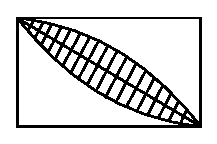
\includegraphics{vol70-figures/fig1.eps}}
\caption{A proper set}
\end{figure}

\setcounter{defi}{22}
\begin{defi}\label{chap4:sec4:def4.23} %4.23
  An operator $T: C^{\infty}_o (\Omega) \to C^{\infty}(\Omega)$ is said
  to be \textit{ properly supported}, if its distribution kernel $K$ has
  proper support. 
\end{defi}

\begin{exercise}
  Let $T = \sum a_{\alpha}(x) D^{\alpha}$ be a differential operator on
  $\Omega$. Computer the distribution kernel $K$ of $T$ and show that
  supp $K$ is a subset of the diagonal. Thus $T$ is properly supported. 
\end{exercise}

If $T$ is properly supported then it maps $C^{\infty}_o$ into itself,
since supp $Tu \subset \pi_1 (\pi^{-1}_2 (\supp u) \cap  \supp K$),
as is easily seen from the formula $Tu(x) = \int K(x,y) u(y) dy$. More
generally, for any $\Omega' \subset \subset \Omega$, there exists
$\Omega'' \subset \subset \Omega$ such that the values of $Tu $ on
$\Omega'$ depend  only on the values of $u$ on $\Omega''$ namely,
$\Omega'' = \pi_2(\pi^{-1}(\Omega') \cap  \supp K$). From this it
follows that $T$ can be extended to a map from $C^{\infty}(\Omega)$ to
itself. In fact, if $u \epsilon C^{\infty}(\Omega)$ and $\Omega',
\Omega''$ are as above, we define Tu on $\Omega'$ by  
$$
Tu|_{\Omega'} = T(\phi u) |_{\Omega},
$$
where $\phi \epsilon C^{\infty}(\Omega)$ and $\phi = 1$ on
$\Omega''$. This definition is independent of\pageoriginale the choice
of $\phi$ and 
gives the same result on the intersection of two $\Omega ' s$; so $Tu$
is well defined on all of $\Omega$. 

If $T$ is a properly supported pseudo differential operator, so that
$T$ extends to a map from $E' (\Omega)$ to $\mathcal{D'}(\Omega)$, the
same arguments show that $T$ maps $E'(\Omega)$ into itself
and extends further to a map of $\mathcal{D'}(\Omega)$ to itself. 

Suppose $T$ and $S$ are properly supported operators on $C^{\infty}
(\Omega)$ with distribution kernels $K$ and $L$ which are  $C^\infty$
off the diagonal. Then $TS$ is an operator on $C^ \infty (\Omega)$
with distribution kernel $M$ formally given by $M(x,y)= \int K (x,z)L
(z,y)dz$. In fact, if $x \neq y$, since $K(x,.)$ and $L(.,Y)$ are
smooth except at $x$ and $y$, the product $K(x,.)L(., Y)$ is a well
defined element of $E'$, and the formula $M(x,y)=<K(x,.)L(.,y),1 >$
displays $M$ as a $C^ \infty$ function off the diagonal. 

\setcounter{prop}{23}
\begin{prop}\label{chap4:sec4:prop4.24} %4.24
  $\Supp M$ is proper. Thus, $TS$ is properly supported.
\end{prop}

\begin{proof}
  Clearly,

  $\Supp M \subset \{ (x,y): \pi _2 (\pi _1^{-1}(x)\cap \supp K) \cap
  \pi_1 (\pi^{-1}_2 (y) \cap \supp L) \neq \phi \}$ Suppose $A \subset
  \Omega$ is compact and set $B= \pi_2 (\pi ^{-1}_1 (A) \cap \supp K)$,
  then $B$ is compact and 
  \begin{align*}
    \pi_1^{-1}(A) \cap \supp M &\subset A \times \left\{ y: B \cap \pi_1 (\pi
    ^{-1}_2 (y)\cap \supp L) \neq \phi \right\}\\
    &= A \times \left\{ y:\pi^{-1}_1 (B) \cap \pi ^{-1}_2 (y) \cap \supp L
    \neq \phi \right\}\\ 
    &= A \times \pi _2 (\pi ^{-1}_1 (B) \cap \supp L)
  \end{align*}
  which is compact. Likewise $\pi ^{-1}_2 (A)\cap \supp M$ is also compact.
\end{proof}

\begin{exercise}
  Suppose\pageoriginale $A \subset (\Omega \times \Omega)$ is proper.  Show that there
  exists a properly supported $\phi \epsilon C^ \infty (\Omega \times
  \Omega)$ such that $\phi =1$ on $A$. (Hint: Let $\{ \phi _j \} \subset
  C^\infty_o (\Omega \times \Omega)$ be a partition of unity on
  $\Omega \times \Omega$ and let $\phi = \sum\limits_{A \cap \supp
    \phi_j}=\phi^{\phi_j}$). 
\end{exercise} 

\section{$\psi do's$ Defined by Multiple Symbols}\label{chap4:sec5} %sce 5

We have arranged our definition of pseudo differential operators to
agree with the usual convention for differential operators, according
to which differentiations are performed first, followed by
multiplication by the coefficients. However, in some situations (for
example, computing adjoints), it is convenient to have a more flexible
setup which allows multiplication operators both before and after
differentiations. We therefore, introduce the following apparently
more general class of operators\break  (which, however, turns out to coincide
with the class of $\psi DO$, modulo smoothing operators). 

\setcounter{defi}{24}
\begin{defi}\label{chap4:sec5:def4.25}%def 4.25
  For $ \Omega $ open in $\mathbb{R}^n$ and $m$ real, we define the {
    \em class of multiple symbols of order $m$ on $\Omega $,} 
  $$
  S^m(\Omega \times \Omega)= \{ a \epsilon C^ \infty (\Omega \times
  \mathbb{R}^n \times \Omega):\forall \alpha, \beta, \forall
  \Omega' \subset \subset \Omega, \exists c=c_{\alpha \beta \Omega '}  
  $$
  such that $\sup\limits_{x,y \epsilon  \Omega'} |D^{\beta}_{x,y} D^
  \alpha _\xi a (x, \xi, y)|\leq  c(1+|\xi|)^{m-|\alpha|} \}$ 
\end{defi}

When $a \epsilon S^m (\Omega \times \Omega)$ we define the operator
$A =a(x,D,y)$ by  
$$
Au (x)= \iint e^{2 \pi i (x-y).\xi}a (x,\xi,y)u(y)dy d \xi
$$

Here the integral must be interpreted as an iterated integral with
integration performed first in $y$ then in $\xi$ as it is not
absolutely convergent as a double integral. 

We\pageoriginale observe that if $a(x, \xi,y)=a (x, \xi)$ is independent of $y$,
then $A=a(x,D)$; thus this class of operators include the $\psi
DO's$. We also observe that different $a's$ may give rise to same
operator. For example, if $a(x,\xi,y)=\phi (x)\psi (y)$ with
$\psi,\phi \epsilon C^\infty_o (\Omega)$ and $\supp \psi \cap \supp\phi
=\phi$, then $a \epsilon s^o(\Omega \times \Omega)$ and
$a(x,D,y)=0$. 

\setcounter{defi}{25}
\begin{defi}%def 4.26
  Given $a \epsilon S^m (\Omega \times \Omega)$ we define
  $$
  \sum_a=\{ (x,y) \epsilon \Omega \times \Omega :(x, \xi,y) 
  \epsilon \supp  \text{ a for some } \xi \epsilon \mathbb{R}^n
  \}. 
  $$
\end{defi}

\setcounter{prop}{26}
\begin{prop}%pro 4.27
  Let $a \epsilon S^m (\Omega \times \Omega)$ and let $K$ be the
  distribution kernel of $A=a(x,D,y)$. Then

  \begin{enumerate}[i)]
  \item $\Supp K \subset \sum_a$, and 
  \item if the support of $K$ is proper, then there exists $a'
    \epsilon S^m (\Omega \times \Omega)$ such that $a'(x,\xi,y)=a(x,
    \xi,y)$ when $(x,y)$ is near the diagonal in $\Omega \times \Omega,
    \sum_{a,}$ is proper and $a(x,D,y)=a' (x,D,y)$. 
  \end{enumerate}
\end{prop}

\begin{proof}
  The kernel $K$ is given by
  $$
  <K,w>= \iiint e^{2 \pi i (x-y). \xi} a (x,\xi, y)w (x,y)dy d\xi dx.
  $$
  
  From this, we see that $<K,w>.=0$ whenever $\supp w \cap
  \sum_a=\phi$. Therefore, $\supp K \subset \sum_a$. This proves (i). 
\end{proof}

To prove (ii), choose a properly supported $\phi \epsilon C^
\infty (\Omega \times \Omega)$ with $\phi =1$ on $\Delta \cup \supp K$,
$\Delta$ being the diagonal. Set $a(x, \xi, y)= \phi (x,y)a (x,
\xi, y)$. Then $\sum_a, \subset  \supp \phi$ and hence $\sum_a$, is
proper. Also $a'(x, \xi, y)= a(x, \xi,y)$ when $(x,y)$ is near the
diagonal. Now, 
\begin{align*}
  <a (x,D,y)u,v> &= <K,v \otimes u>\\
  &= < \phi K,v \otimes u>\\
  &= < K, \phi (v \otimes u)>\\
  &= \iiint e^{2 \pi i (x-y)\cdot \xi} a (x, \xi, y) \phi (x,y) \times v(x)u
  (y)dy d \xi dx\\ 
  &= \iiint e^{2 \pi i (x-y). \xi}a' (x, \xi, y)u(y)dy d \xi dx \\
  &= <a'(x,D,y)u,v>.
 \end{align*}\pageoriginale
 
Since $v$ is arbitrary, we have $a (x,D,y)=a'(x,D,y)$.

\setcounter{thm}{27}
\begin{thm}\label{chap4:sec5:thm4.28}%the 4.28
  Suppose $a \epsilon S^m (\Omega \times \Omega)$ and $A=a
  (x,D,y)$ is properly supported. Let $p(x, \xi)=e^{-2 \pi i x.\xi}
  A(e^{2 \pi i(.). \xi})(x)$. Then $p \epsilon S^m (\Omega)$ and $p
  (x,D)=A$. Further, 
  $$
  p(x,\xi) \sim \sum_a \frac {1}{\alpha !} \partial ^ \alpha _ \xi D^
  \alpha _y a (x, \xi, y)|_{y=x}. 
  $$ 
\end{thm}

\begin{proof}
  For u in $C^ \infty _o (\Omega)$, we have 
  $$
  u(x)= \int e^{2 \pi ix. \xi} \hat {u}(\xi)d \xi.
  $$
    
  Therefore, by linearity and continuity of $A$,
  \begin{align*}
    Au (x)&= \int A (e^{2 \pi i (.). \xi}) (x) \hat{u}(\xi)d \xi \\
    &= \int e^{2 \pi i x. \xi}p (x, \xi) \hat{u}(\xi)d \xi =p (x,D)u (x).
  \end{align*}
\end{proof}
 
 By the proposition above, we can modify a so that $\sum_a$ is proper
 without affecting $A$ or the behaviour of a along the diagonal $x=y$
 (which is what enters into the asymptotic expansion of $p$). Set $b(x, \xi
,y)=a (x, \xi, x+y)$.\pageoriginale Then as a function of $y,b$ has compact
 support. Indeed, for fixed $x$ and $\xi$, if $y \epsilon \{ y':
 b(x, \xi,y') \neq 0 \}$ then $x+y \epsilon \pi_2 (\pi ^{-1}_1 (x)
 \cap \sum_a)$ which is compact. Now, 
 \begin{align*}
   p (x, \eta) &= e^{-2 \pi i x. \eta} \iint e^{2 \pi i (x-y). \xi} b(x,
   \xi, y -x)e^{2 \pi i y. \eta} dy d \xi\\ 
   &= e^{-2 \pi i x. \eta} \iint e^{2 \pi i z. \xi}b (x, \xi z) e^ {2
     \pi i (z+x). \eta } dz d \xi \\ 
   &= \int \hat{b}_3 (x, \xi, \xi- \eta)d \xi = \int \hat{b}_3 (x, \xi
   + \eta,  \xi)d \xi, 
 \end{align*} 
 where $\hat{b}_3$ is the Fourier transform of $b$ in the third
 variable. Since $b(x, \xi,.)$ is in $C^ \infty _o$, this calculation
 is justified and $\hat{b}_3 (x, \eta, \xi)$ is rapidly decreasing in
 the variable $\xi$. 
  
 More precisely, since $a \epsilon S^m (\Omega \times \Omega)$, we have 
 \begin{equation}
   | D^\beta _x D^\alpha _\eta \hat{b}_3 (x, \eta, \xi) | \le c_{ \alpha
     \beta N} (1+| \eta |)^{m-| \alpha |}
   (1+|\xi|)^{-N}.\tag{4.29}\label{chap4:sec5:eq4.29}  
 \end{equation} 
 
 Since
$$
\left(\frac {1+|\eta|} {1+|\xi|} \right)^s \le (1+|\xi-
\eta|)^{|s|}, \text{ taking } \eta + \xi \text{ instead of } \eta 
$$
we have $(1 + |\xi+ \eta |)^s \le (1+ |\xi|)^s (1+ |\eta|)^{|s|}$. If
we use this in  
 $$
 |D^\beta _x D^\alpha _\eta \hat{b}_3 (x, \xi + \eta, \xi)| \le
 c_{\alpha \beta N}(1+|\xi+ \eta|)^{m-|\alpha|}(1+|\xi|)^{-N} 
 $$
 we get
 $$
 |D^\beta _x D^\alpha _\eta \hat{b}_3 (x, \xi + \eta, \xi)| \le
 c'_{\alpha \beta N}(1+|\xi|)^{-N+m-|\alpha|}(1+
 |\eta|)^{|m|+|\alpha|}. 
 $$
  
If we take $N$ so that $-N+m -|\alpha| <-n$ we have
\begin{align*}
  |D^\beta _x D^ \alpha _ \eta p (x, \eta)| & = |\int D^\beta _x D^ \alpha
  _ \eta \hat{b}_3 (x, \xi+ \eta,  \xi) d \xi|
  \tag{4.30}\label{chap4:sec5:eq4.30} \\
  & \leq c_{\alpha \beta}(1+|\eta|)^{|m|+|\alpha|}
\end{align*}
 
 On\pageoriginale the other hand, taking the Taylor expansion of
 $\hat{b}_3 (x, \xi  + \eta,  \xi)$ in the middle argument about the
 point $\eta$, (\ref{chap4:sec5:eq4.29}) gives  
\begin{align*}
  |\hat{b}_3 (x, \xi + \eta, \xi) & - \sum_{|\alpha|< k} \partial
  ^{\alpha}_\eta \hat{b}_3 (x, \eta, \xi) \frac {\xi ^\alpha}{\alpha
    !}| \\
 & \le C|\xi|^k \sup_{\substack {|\alpha|=k \\{0 \le t \le 1}}}
  |\partial ^\alpha _ \eta \hat{b}_3 (x, \eta + t \xi,  \xi)|\\ 
  &  \le C_N |\xi|^k  \sup_{0 \le t \le 1} (1+|\eta +t
  \xi|)^{m-k}(1+|\xi|)^{-N}. 
\end{align*}

When $|\xi| <\frac{1}{2} |\eta|$, taking $N=k$ we get
$$
|\hat{b}_3 (x, \xi + \eta, \xi)- \sum_{|\alpha|< k} \partial ^ \alpha_
\eta \hat{b}_3 (x, \eta,  \xi) \frac{\xi^\alpha}{\alpha !}| \le c_k
(1+|\eta|)^{m-k}. 
$$

When $|\xi| \ge \dfrac{1}{2}|\eta|$, we have
$$
|\hat{b}_3 (x, \xi +\eta, \xi)- \sum_{|\alpha|< k} \partial ^{\alpha}_
\eta \hat{b}_3 (x, \eta, \xi) \frac {\xi^\alpha}{\alpha !}|\le C_N
(1+|\xi|)^{m+k-N}.  
$$

(Actually, the exponent of $(1+|\xi|)$) can be taken as $m-N$ when
$m-k \ge 0$ and when $m-k < 0)$. Also we have 
\begin{align*}
  \int \partial^\alpha_\eta \hat{b}_3 (x, \eta, \xi) \xi^\alpha d \xi
  &= D^\alpha_Y \int e^{2 \pi i Y \cdot \xi} \partial^\alpha_\eta
  \hat{b}_3 (x,\eta, \xi)d \xi |_{Y=0}\\ 
  &= D^\alpha_Y \partial^\alpha_ \eta b(x, \eta, y)|_{Y=0}\\
  &= D^\alpha_Y \partial^\alpha_\eta a(x, \eta, y)| _{y=x}.
\end{align*}

So finally
\begin{align*}
  |p(x, \eta) & - \sum _{|\alpha| <k} D^ \alpha _y \partial ^ \alpha _ \eta
  a (x, \eta, y) \frac {1}{\alpha !}|_{y=x}| \\
  &= |\int \hat{b}_3 (x, \xi + \eta,  \xi) d \xi -\sum_{|\alpha|< k}
  \frac {1}{\alpha !} \int \partial ^ \alpha _ \eta \hat{b}_3 (x, \eta
  , \xi) \xi^{\alpha}d \xi| \\ 
  & \le C_k \int \limits_{|\xi|< \frac {|\eta|}{2}} (1+ |\eta|)^{m-k} d
  \xi+ C_N \int \limits _{|\xi| \ge \frac{|\eta|}{2}} (1+
  |\xi|)^{m+k-N} d \xi. 
\end{align*}

Now\pageoriginale
$$
\int\limits_{|\xi|< \frac{|\eta|}{2}} C_k (1+ |\eta|)^{m-k} d \xi=
C'_k (1+|\eta|)^{m-k} |\eta|^n \le C'_k (1+ |\eta|)^{m-k+n} 
$$

In the second integral, we take $N > n +m + k$ so that 
$$
\int \limits_{|\xi|^ \ge \frac{|\eta|}{2}}C_N (1+ |\xi|)^{m-N} d \xi
\le C'_N (1+|\eta|)^{m-N+n}, 
$$
by the usual integration in polar coordinates. Therefore, since $N \ge
k$ we obtain 
$$
|p (x, \eta)- \sum_{|\alpha|<k} \frac {1}{\alpha !} D^{\alpha }_y
\sigma ^\alpha _\eta a(x, \eta, y)|_{x=y}|\le C_k (1+ |\eta|)|^
       {\mu_k} 
$$
with $\mu _k=m-k+n$.

Combining this with (\ref{chap4:sec5:eq4.30}), we see that all the conditions of
Theorem \ref{chap4:sec3:thm4.20} are satisfied, so we are done. 

\setcounter{coro}{30}
\begin{coro}\label{chap4:sec5:coro4.31}%coro 4.31
  If $P \epsilon \psi ^m$, there exists a $Q \epsilon \psi^m$
  such that $Q$ is properly supported and $P - Q$ is smoothing. 
\end{coro}

\begin{proof}
  If $P= p(x,D)$ choose $\phi \epsilon C^ \infty (\Omega \times
  \Omega)$ which is properly supported and $\phi =1$ near the
  diagonal. Set $a(x, \xi, y)= \phi (x,y)p (x,\xi)$. Then $a \epsilon
  S^m (\Omega \times \Omega)$ and by construction $\sum_a$ is proper. So
  $a(x,D,y)= Q \epsilon \psi ^m$. If $K_p$ and $K_Q$ denote the
  distribution kernels of $P$ and $Q$ then it is easily seen that $K_Q=
  \phi K_p$. This shows that $K_Q- K_p$ vanishes near the diagonal: so,
  by Theorem \ref{chap4:sec2:thm4.10}, $K_ Q- K_p$ is $C^
  \infty$. Therefore, $Q-p$ is smoothing. 
\end{proof}

\setcounter{rem}{31}
\begin{rem}\label{chap4:sec5:rem4.32}%rem 4.32
  The idea of multiple symbols can clearly be generalised. For example,
  if $a \epsilon C^ \infty (\Omega \times \mathbb{R}^n \times \Omega
  \times \mathbb{R}^n)$ satisfies estimates of the form $|D^v_{x,y} D^ \alpha _
  \xi D^ \beta _ \eta a(x, \xi, y, \eta)| \le C (1+ \eta|)^{m_2
    -|\beta|} (1+ |\xi|)^{m_1-|\alpha|}$,\pageoriginale  one can
  define an operator $A=a(x,D,y,D)$ by 
\end{rem}
$$
Au (x)= \iiint e^{2 \pi i(x. \xi-y. \xi+y. \eta)} a (x,\xi, y, \eta)
\hat{u}(\eta) d \eta dy d \xi 
$$
which agree with our previous definitions, if a is independent of the
last one or two variables. As one would expect, under reasonable
restriction on $\supp a$, it turns out that $A \epsilon \psi
^{m_1+m_2}(\Omega)$. The reader may wish to amuse himself by working
this out and computing the symbol of $A$. 

\section{Products and Adjoint of $\psi DO'S$}\label{chap4:sec6}%sce 6

We are now in a position to compute products and adjoints of $\psi
DO'S$. First we clarify our terminology. Let $T$ $S$ be linear
operators from $C^\infty_o (\Omega)$ into $C^\infty (\Omega)$. We
say that $S=T^t$ if $<Tu,v>= <u,Su>$ for $u,v \epsilon C^\infty _o
(\Omega)$ and we say that $S=T^*$ if $<Tu, \bar{v}>=<u, \bar {Sv}>$
for $u,v \epsilon C^ \infty _o (\Omega)$. 

\setcounter{rem}{32}
\begin{rem}\label{chap4:sec6:rem4.33}%rem 4.33
  If $T$ is properly supported, then $T^t$ and $T^*$ are also properly
  supported. Indeed, if $K$ is the distribution kernel of $T$, then the
  distribution kernel of $T^t$ is $K^t$ and that of $T^*$ is $K^*$ where
  $K^t (x,y)=K(y,x)$ and $K^*(x,y)= K (\overline {y,x})$. 
\end{rem}

We recall that if $P \epsilon \psi ^m (\Omega)$, we denote the
corresponding symbol in $S^m (\Omega)$ by $\sigma _p$. 

\setcounter{thm}{33}
\begin{thm}\label{chap4:sec6:thm4.34}%the 4.34
  If $P \epsilon \psi ^m(\Omega)$ is properly supported, then
  $P^t, P^* \epsilon \psi ^m (\Omega)$ and $\sigma _p t(x, \xi) \sim
  \sum \limits_{\alpha}\dfrac {(-1)^{|\alpha|}}{\alpha !} \partial
  ^\alpha _\xi D^ \alpha _x \sigma _p (x,- \xi)$, 
  $$
  \sigma _{p^*}(x, \xi)\sim \sum_a \frac {1}{\alpha !}\partial ^\alpha _
  \xi D^ \alpha_x \bar{\sigma}_p (x,\xi). 
  $$
\end{thm}

\begin{proof}
  For\pageoriginale $u,v \epsilon C^\infty _o (\Omega)$, we have 
  \begin{align*}
    <Pu,v> &= \iint e^{2 \pi ix,  \xi} p(x, \xi) \hat {u}(\xi)v (x) d \xi dx\\
    &= \int \left(\int e^{2 \pi ix,  \xi} p(x, \xi)v (x) dx\right)
    \hat {u}(\xi)d \xi\\ 
    &=\int g (\xi) \hat{u}(\xi) d \xi
  \end{align*}
  where 
  $$
  g(\xi)= \int e^{2 \pi ix,  \xi} p(x, \xi)v(x)dx.
  $$
\end{proof}

By Corollary \ref{chap4:sec1:coro4.6}, $g$ us a rapidly decreasing
function. Thus 
$$
<Pu,v>= \int g \hat {u}= \int u \hat{g}=<u, P^t_v>
$$
so that
\begin{align*}
  P^tv (y)= \hat{g}(y) &= \iint e^{2 \pi i (x-y). \xi} p(x, \xi) v (x)dx
  d \xi \tag{4.35} \label{chap4:sec6:eq4.35}\\ 
  & = \iint e^{2 \pi i (y-x). \xi}p(x,- \xi) v (x)dx d \xi \\
  &=a(x,D,y)v (y)
\end{align*} 
where $a (x, \xi y)=p(y.-\xi)$. Therefore, by Theorem
\ref{chap4:sec5:thm4.28},    
  $$
  P^t \epsilon \psi ^m (\Omega) ~\text{and}~ \sigma _{P^t}(x,\xi)
  \sim \sum _a \frac{(-1)^{|\alpha|}}{\alpha !} \partial ^ \alpha _\xi
  D^\alpha _x \sigma _P (x, -\xi). 
  $$  
  
  The assertions about $P^*$ follows along similar lines
\setcounter{thm}{35}
\begin{thm}\label{chap4:sec6:thm4.36}%the 4.36
  If $P \epsilon \psi^{m_1}(\Omega)$ and $Q \epsilon
  \psi^{m_2}(\Omega)$ are properly supported, then $QP \epsilon
  \psi^{m_1+m_2}(\Omega)$ and 
  $$
  \sigma_ {QP}(x,\xi)  \sim \sum_{\alpha} \frac{1}{ \alpha !}\partial
  ^\alpha _ \xi \sigma _{Q} (x, \xi) D^ \alpha _x \sigma_p (x,\xi). 
  $$
\end{thm}

\begin{proof}
  Since\pageoriginale $P = (P^t)^t$, we have
  $$
  (Pu) (x) = \iint e^{2 \pi i (x-y)\cdot \xi} \sigma_P^t (y, - \xi) u
  (y) dy d\xi 
  $$
  \text{by} (\ref{chap4:sec6:eq4.35}).  
\end{proof}

In other words
$$
(Pu)\hat{~} (\xi) = \int e^{-2 \pi i y\cdot \xi} \sigma_{P^t} (y,  -xi) u (y) dy.
$$

Therefore,
\begin{align*}
  (QP) u(x)  & = \iint e^{2 \pi i (x-y)\cdot \xi} \sigma_Q (x,  \xi)
    \sigma_{P^t} (y,  -xi) u(y) dy d\xi\\ 
  & = a(x,D,y) u(x)
\end{align*}
where $a (x, \xi,  y) = \sigma_{Q} (x, \xi )\sigma _{P^t} (y, 
-\xi)$. Clearly  $a \epsilon S^{m_1 + m_2} (\Omega  \times \Omega)$
which implies $QP \epsilon \psi^{m_1 + m_2} (\Omega)$. Moreover 
\begin{align*}
  \sigma_{Q P} (x,  \xi) & \sim \sum_\alpha \frac{1}{\alpha!}
  \partial^{\alpha}_{\xi}D^{\alpha}_{y}(\sigma_Q (x,  \xi) \sigma_{p^t} (y,-\xi
  ))|_{y=x}\\ 
  & \sim \sum_{\alpha} \frac{1}{\alpha!} \sum_{\beta + \nu = \alpha }
  \frac{\alpha}{\beta !\nu!} \partial^{\beta}_{\xi} \sigma_{Q}(x, \xi)
  \partial^{\nu}_{\xi} D^{\alpha}_Y \sigma_{P^t}(x,-\xi)\\ 
  & \sim \sum_{\alpha,\nu} \sum_{\delta} \frac{(-1)^{|\delta|}}{\nu !
    \beta ! \delta!}\partial^{\beta}_{\xi}\sigma_{{Q}}(x, \xi)
  D^{\beta+ \nu + \delta} \partial^{\nu + \delta}_{x} \partial^{ \nu +
    \delta}_{\xi}\sigma_{P}(x,-\xi)\\ 
  & \sim \sum_{\beta,  \lambda} \left( \sum_{\nu + \delta =
    \lambda}\frac{(-1)^{|\delta|}}{\nu ! \beta ! \delta!}\right)
  \frac{1}{\beta!}\partial^{\beta}_{\xi}\sigma_{Q}(x, \xi)
  D^{\beta+\lambda}_{x} \partial^{\lambda}_{\xi} \sigma_p(x,\xi) 
\end{align*}

But $\sum \limits _{v+ \delta =\lambda} \frac{(-1)^{|\delta|}}{v!
  \delta !}= (x_0-x_0)^\lambda$ with $x_0=(1,1, \ldots, 1)$ 
\begin{equation*}
  =
  \begin{cases}
    1 ~\text{ if }~ \lambda ~ = ~ 0 \\ 
    0 ~\text{ if } ~\lambda ~\neq ~ 0
  \end{cases}
\end{equation*}

Therefore $\sigma _{QP}(x, \xi) \sim \sum\limits_\beta
\dfrac{1}{\beta !} \partial^{\beta}_{\xi} \sigma_Q (x,
\xi)D^\beta_x \sigma_p (x, \xi)$. 

\setcounter{coro}{36}
\begin{coro}[PRODUCT RULES FOR $\psi DO'S$]\label{chap4:sec6:coro4.37}
~  

If\pageoriginale  $Q= q (x,D) \epsilon \psi
  ^m (\lambda)$ and $f \epsilon C^\infty (\Omega)$, then for any
  positive integer $N$, $q(x,D)(fu)= \sum \limits _{|\alpha|<N}
  \dfrac{1}{\alpha !} D^ \alpha f [(\partial ^\alpha_\xi
    q)(x,D)u]+T_Nu$ where $T_N \epsilon \psi^{m-N}(\Omega)$. 
\end{coro}

\setcounter{coro}{37}
\begin{coro}\label{chap4:sec6:coro4.38}%coro 4.38
  The correspondence $p \to p(x,D)$ and $P \to \sigma_p$ are *
  homomorphisms modulo lower order term i.e., if $p \epsilon
  S^{m_1}(\Omega)$ and $q \epsilon S^{m_2}$ $(\Omega)$, then
  $(pq)(x,D)- p(x,D)q(x,D) \epsilon \psi^{m_1 +m_2-1}(\Omega)$ and
  $p (x,D)^*-\bar{p}(x,D)$ $\epsilon \psi ^{m_1-1}$ and also, if $P
  \epsilon \psi ^{m_1}(\Omega) $ and $Q \epsilon
  \psi^{m_2}(\Omega)$, then $\sigma_{P Q} -\sigma_P \sigma_{Q}\break
  \epsilon S^{m_1+m_2-1}$ $(\Omega)$, $\sigma_{P*}-\bar{\sigma}+p
  \epsilon S^{m_1-1} (\Omega)$.
\end{coro}

\begin{coro}\label{chap4:sec6:coro4.39}%coro 4.39
  If $P \epsilon \psi ^{m_1}(\Omega)$ and $Q \epsilon
  \psi^{m_2}$ $(\Omega)$, then $[P,Q]=P Q-QP$ $\epsilon$ $\psi^{m_1m_2-1}
  (\Omega)$ and $\sigma_{[P, Q]}- \dfrac {1}{2 \pi i} \{ \sigma_P
 , \sigma _ {Q}\}  \epsilon S^{m_1m_2-1}(\Omega)$ where $\{ f,q \}$
  stands for the Poisson bracket defined by  
  $$
  \{ f, q \} = \sum \left(\frac {\partial f}{\partial \xi_j}\frac {\partial
    g}{\partial x_j} - \frac {\partial f}{\partial x_j}\frac {\partial
    g}{\partial \xi_j}\right). 
  $$
\end{coro}
Following the philosophy that smoothing operators are negligible it is
a trivial matter to extend these results to non-properly supported
operators. 

Suppose $P \epsilon \psi ^m (\Omega)$ is not properly
supported. By corollary \ref{chap4:sec5:coro4.31}, we can write $P=P_1+s$ where $P_1$ is
properly supported and $S$ is smoothing. Then $P^t=P^t_1+S$ where
$P_1^t$ is given by Theorem \ref{chap4:sec6:thm4.34} and $S^t$ is
again smoothing 
(c.f. Remark \ref{chap4:sec6:rem4.33}). Likewise for $P^*$. If $Q$ is a properly
supported $\psi DO$, the products $P Q$ and $QP$ are well defined as
operators from $C^ \infty _o (\Omega)$ to $C^\infty (\Omega)$. Again,
we have $P Q= P_1 Q+S Q$ and $QP= QP_1+ Qs; P_1 Q$ and $QP_1$ are
described by Theorem \ref{chap4:sec6:thm4.36}, while $SQ$ and $QS$ are
smoothing.  

\section[A Continuity Theorem for $\psi$ Do on Sobolev
  Spaces]{A Continuity Theorem for $\psi$ Do on Sobolev\hfill\break
  Spaces}\label{chap4:sec7} %sec 7

We\pageoriginale now state and prove a continuity theorem for pseudo defferential
operators acting on Sobolev spaces. We are indebted to Dr
P.N. Srikanth for simplifying our original argument. 
\setcounter{thm}{39}
\begin{thm}\label{chap4:sec7:thm4.40}%the 4.40
  Suppose $P=p(x,D)\epsilon \psi ^m (\Omega)$. Then
  \begin{enumerate}[\rm i)]
  \item $P: H_s \to H^{\loc}_{s-m}(\Omega)$ continuous for all
    $s \epsilon \mathbb{R}$. 
  \item If $P$ is properly supported, $P: H^{\loc}_s (\Omega) \to
    H^{\loc}_{s-m}(\Omega)$ continuously for all $s \epsilon
    \mathbb{R}$ 
  \end{enumerate}
\end{thm}

\begin{proof}
To established (i), we must show that the map $u \to \phi Pu$ is
bounded from $H_s \to H_{s-m}$ for any $\phi \epsilon C^\infty _o
(\Omega)$. Replacing $p (x, \xi)$ by $\phi (x)p (x, \xi)$ we must
show: 
\end{proof}

\noindent  (4.41)\qquad 
if $p \epsilon s^m (\mathbb{R})$ and $p(x, \xi)=0$ for $x$ outside
a compact set, then $p=p(x,D)$ is bounded from $H_s$ and $H_{s-m}$ for
every $s$ in $\mathbb{R}$. 

Suppose then that $u \epsilon H_s$. Then $pu \epsilon E'$, and
from the definition of $P$ on distributions, we see that 
\begin{align*}
  (Pu)^{\hat{}}(\eta) & = < Pu, e^{-2 \pi i \eta.(.)}>\\
  &=\iint e^{2 \pi i (\xi- \eta). x} p(x, \xi) \hat{u}(\xi ) dx d \xi\\
  &= \int \hat{p}_1 (\eta - \xi, \xi) \hat{u}(\xi)d \xi 
\end{align*}
and hence, if $V \epsilon S$, 
\begin{align*}
  <Pu, \bar{v}> & = \int (Pu)^{\hat{}}\hat{v}= \iint K(\eta,  \xi)f
  (\xi)\bar{g}(\eta) d \xi d \eta\\
  \text{where} \hspace{2cm} f(\xi) & = (1 +|\xi|^2)^{s/2} \hat{u}(\xi)\\
  g (\eta) &= (1 + |\eta|^2)^{(m-s)/2} \hat{v}(\eta)
\end{align*}
and $K(\eta, \xi) = \hat{p}_1 (\eta - \xi, \xi) (1+ |\xi|^2)^{-s/2}
(1+ | \eta|^2)^{(s-m)/2}$.\pageoriginale 

We wish to estimate $K(\eta, \xi)$. For any multi-index $\alpha$,
since\break $p(., \xi) \epsilon C^{\infty}_o$, we have  
\begin{align*}
  |\zeta^{\alpha} \hat{p}_1(\zeta, \xi)| & = | \int (D^{\alpha}_x e^{-2
    \pi i x. \zeta)} p( x, \xi)dx | \\ 
  & = | \int  e^{-2 \pi i x. \zeta)} (D^{\alpha}_x p( x, \xi)dx| \\
  & \leq C_{\alpha}(1+ |\xi| )^m,
\end{align*}
so that for any positive integer $N$,
$$
|\hat{p}_1 (\zeta, \xi)| \leq C_N(1+ | \xi |)^m (1+ | \zeta|)^{-N}
$$
and hence
\begin{align*}
  | K(\eta, \xi)| & \leq C_N(1+ | \xi |)^{m-s}(1+ | \eta|)^{s-m}(1+|\xi -
  \eta|)^{N} \\ 
  & \leq C_N(1+ | \xi |)^{|m-s|-N}
\end{align*} 
If we take $N> n+ |m-s|$, we see that 
$$
\int | K(\eta, \xi)| d \eta \leq C, \int |K(\eta,  \xi)| d \xi \leq C.
$$

Therefore by Theorem \ref{chap1:sec1:thm1.1} and the Schwarz inequality,
$$
| < Pu, \bar{v}> | \leq C|| f||_2 ||g||_2 = C|| u||_{(s)} ||v||_{(m-s)}.
$$

From this, it follows that $||Pu||_{(s-m)} \leq C||u||_{(s)}$ for $u
\epsilon H_s$ which establishes (4.41) and hence (i). 

Now suppose $P$ is properly supported and $u \epsilon H^{\loc}_s
(\Omega)$. If $\phi \epsilon C^{\infty}_o (\Omega)$ there exists
$\Omega' \Subset \Omega$ such that the values of Pu on $\supp \phi$
depend only the values of $u$ on $\Omega$. Thus if we pick $\phi'
\epsilon C^{\infty}_o (\Omega)$ with $\phi' = 1$ on $\Omega'$, we
have $\phi Pu = \phi P(\phi 'u)$. But $\phi' u \epsilon H_s$\pageoriginale and
(4.41) $\phi P$ is bounded from $H_s$ to $H_{s-m}$. This establishes (ii)
and completes the proof. 

\section{Elliptic Pseudo Differential Operators}\label{chap4:sec8}%sec 8

\setcounter{defi}{41}
\begin{defi}\label{chap4:sec8:def4.42}%4.42
  $P \epsilon \psi^m (\Omega)$ is said to be \textit{ elliptic of
    order } $ m$ if $| \sigma_P (x, \xi)| \geq C_{\Omega}, |\xi|^m$
  for large $|\xi|$, for all $x \epsilon \Omega', \Omega' \Subset
  \Omega$. 
\end{defi}

\begin{defi}\label{chap4:sec8:def4.43}%4.43
  If $P \epsilon \psi^m (\Omega)$,  a {\em left (resp. right )
    parametrix of } $P$ is a $\psi D O Q$ such that $QP -I$(resp. PQ -I)
  is smoothing. 
\end{defi}

\setcounter{thm}{43}
\begin{thm}\label{chap4:sec8:thm4.44}%4.44
  If $P \epsilon \psi^m $ {\em is elliptic of order $m$ and properly
  supported, then there exists a properly supported $ Q \epsilon
  \psi^{-m}$ which is a two-sided para\-metrix for $P$}. 
\end{thm}

\begin{proof}
  Let $P = p(x,D)$. We will obtain $Q = q(x,D)$ with $q \sim \sum
  \limits^{\infty}_{j=0} q_j$ where the $q_j'$s are defined recursively.
  Let $\zeta (x, \xi)$ be a $C^{\infty}$ function such that $\zeta (x,
  \xi)=1$ for large $\xi$ and $\zeta (x, \xi)= 0$ in a neighbourhood of
  the zeros of $p$. Define $q_o (x, \xi) =\dfrac{\zeta (x, \xi)}{p(x,
    \xi)}$.  Then $q_o \epsilon s^{-m}$.  Let $Q_o = q_o (x,D)$. We
  have  
  $$
  \sigma_{Q_O^p} = q_0^p \mod S^{-1}= 1 \mod S^{-1} = 1+ r_1 ~\text{ with }~ r_1
  \epsilon S^{-1}. 
  $$
\end{proof}

Let $q_1 = \dfrac {-r_1\zeta}{p}, Q_1 = q_1 (x,D)$. Then
\begin{align*}
  \sigma_{(Q_0 + Q_1)P} & = \sigma_{Q_O^p}+ \sigma_{Q_1^p} = 1+ r_1 -r_1
  \zeta \mod S^{-2} \\ 
  & = 1+ r_2 ~\text{ with }~ r_2 \epsilon S^{-2}.
\end{align*}

Let $q_1 = \dfrac { ^{-r}2^{\zeta}}{p}$ etc. Having determined $q_1,q_2
, \ldots q_j$ so that  
$$
\displaylines{\hfill
  \sigma_{(Q_0+ Q_1 + \cdots Q_j)P}= 1 + r_{j+1}, r_{j+1} \epsilon
  S^{-(j+1)}\hfill\cr 
  \text{set} \hfill  
  q_{j+1}= \frac{-r_{j+1}\zeta}{p}.\hfill}
$$\pageoriginale

Let $Q$ be a properly supported operator with symbol $q \sim \sum
\limits^{\infty}_{j=0} q_j$. Then $\sigma_{QP}= 1$ mod $S^{-\infty}$,
i.e., $QP- I$ is smoothing. Thus $Q$ is a left parametrix. In the same
way, we can construct a right parametrix $Q'$. Then if $S = QP -I$ and
$S' =PQ'-I$, we have  
$$
QPQ' =SQ'+Q' = QS'+ Q. 
$$

So $Q - Q' = SQ' - QS$' is smoothing. Hence $Q$ is a two sided parametrix.
\begin{exercise}
  What happens if $P$ is not properly supported? (cf. the remarks at the
  end of \S \ref{chap4:sec6}). 
\end{exercise}

The left parametrices are used to prove regularity theorems and the
right parametrices are used to prove existence theorems. 

Indeed, we have:
\setcounter{coro}{44}
\begin{coro}[ELLIPTIC REGUIARITY THEOREM]\label{chap4:sec8:coro4.45}%% coro4.45 
  If $P$ is elliptic of order $m, u
  \epsilon \mathcal{D}' (\Omega), Pu \epsilon
  H^{\loc}_{s}(\Omega)$ implies $u \epsilon
  H^{\loc}_{s+m}(\Omega)$. In particular, $P$ is hypoelliptic. 
\end{coro}

\begin{proof}
  Let $Q$ be a left parametrix and set $S = QP-I$. Then $u = QPu -
  Su$. Since$Pu \epsilon H^{\loc}_{s}(\Omega)$ and $Q$ is properly
  supported, $Q \epsilon \psi^{-m}$ we have $QPu \epsilon
  H^{\loc}_{s+m}(\Omega)$ by Theorem \ref{chap4:sec7:thm4.40}. Also $Su \epsilon
  C^{\infty}$ since $S$ is smoothing. Hence $u \epsilon
  H^{\loc}_{s+m}(\Omega)$. 
\end{proof}

\setcounter{thm}{45}
\begin{thm}\label{chap4:sec8:thm4.46} % the 4.46
  Every elliptic differential operator is locally solvable. In fact,
  if $P$ is elliptic on $\Omega, f \epsilon \mathcal{D}'(\Omega)$
  and $x_o \epsilon \Omega$, there exists\pageoriginale $u \epsilon
  \mathcal{D}'(\Omega)$ such that $Pu =f$ in a neighbourhood of
  $x_o$. (Of course, if $f \epsilon C^{\infty}$, then $u
  \epsilon C^{\infty}$ near $x_o$, by the previous corollary).
\end{thm}

\begin{proof}
  BY cutting $f$ off away from $x_o$, we can assume that $ f \epsilon
  E'$ and hence $ f \epsilon H_s$ for some $s$. Let $Q$ be a properly
  supported parametrix for $P$ and let $S = PQ -I$. Then $S$  is also
  properly supported. If $\Omega_1 \subset \subset \Omega$ is a
  neighbourhood of $x_o$ then there  exists $\Omega_2 \subset \subset
  \Omega$ such that the values of Su on $\Omega_1$ depend only on the
  values of $u$ on $\Omega_2$. Pick $\phi_1, \phi_2 \epsilon
  C^{\infty}_o(\Omega)$ such that $\phi_j \equiv 1$ on $\Omega_j, j =
  1,2$ and set $Tu = \phi_1 S(\phi_2 u)$. 
\end{proof}

Now observe the following :
\begin{enumerate}[i)]
\item $Tu = su $ on $\Omega_1$.
\item $T : H^s \to C^{\infty}_o$(suup $\phi_1)$ continuously.
\end{enumerate}

From (ii) and the Arzela -Ascoli theorem, it follows that if $(u_k)$
is a bounded sequence in $H_{s'} (Tu_k)$ has a convergent subsequence in
$C^{\infty}_o$(suup $\phi_1)$ and hence in $H_s$. Therefore, $T$ is
compact on $H_s$. So the equation $(T + I)u = f$ can be solved if $f$
is orthogonal (with respect to the pairing of $H_s$ and $H_{-s})$ to
the space $N = \{ g : ( T^* + I) g = 0 \}$. This space $N$  is a
finite dimensional space of $C^{\infty}$ functions so we can always
make this happen by modifying $f$ outside a small neighbourhood of
$x_o$. 

Indeed, pick a basis $g_1,g_2,  \ldots,  g_{\nu}$ for $N$ and pick a
neighbourhood $U$  of $x_o$ so small that $g_1, \ldots,  g_{\nu}$ are
linearly independent as functionals on $C^{\infty}_o (\Omega
\backslash U)$. (Such a $U$ exists; otherwise,  by a limiting argument
using the local compactness of $N$, we could find a nontrivial linear
combination of $g_1, \ldots,  g_{\nu}$ supported at $\{ x_o \}$, which
is absurd). Then we can make $f \perp N$ by adding to $f$ a function
in $C^{\infty}_o (\Omega \backslash U)$. But then  
$$
PQu = (I +S) u = (I +T) u \text{ on } \Omega_1 \text{ and } (I +T)u =f
$$\pageoriginale
in a neighbourhood of $x_o$. So $Qu$ solves the problem.

\section{Wavefront Sets}\label{chap4:sec9}%sec 9

We now introduce the notion of wavefront sets, which provides a
precise way of describing the singularities of distributions: it
specifies not only the points at which a distribution is not smooth
but the directions in which it is not smooth. 

All pseudo differential operators encountered in this section will be
presumed to be properly supported,  and by ``$\psi D O$'' we shall
always mean ``properly supported $\psi D O$''. 

\setcounter{defi}{46}
\begin{defi}\label{chap4:sec9:def4.47}%defini 4.47
  \begin{enumerate}[\rm (i)]
  \item Let $\Omega$ be an open set in $\mathbb{R}^n$. Then we define
    $T^o \Omega = \Omega \times (\mathbb{R}^n \backslash \{ 0 \}) $. (In
    coordinate - invariant terms, $T^o \Omega $ is the cotangent bundle
    of $\Omega$ with the zero section removed). 
  \item A set $S \subset T^o \Omega $ is called {\em conic } if $(x,
    \xi) \epsilon S \Rightarrow (x, r \xi) \epsilon S,  \forall r
    > 0$ 
  \item Suppose $P = p(x,D) \epsilon \psi^{m}(\Omega)$. Then $(x_o,
    \xi_o) \epsilon T^o \Omega $ is said to be \textit{
      non-characteristic } for $P$ if $| p ( x, \xi) | \geq c|\xi|^m$
    for $|\xi|$ large and $(x, \xi)$ in some conic neighbourhood of
    $(x_o, \xi_o)$. 
  \item The \textit{ characteristic variety of } $P$, denoted by char
    $P$, is defined by char $P= \{ (x, \xi)  \epsilon T^o \Omega : (x,
    \xi)$ is characteristic for $p$ \}. 
  \item Let $u \epsilon \mathcal{D}' (\Omega)$. The \textit{
    wavefront set} of $u$, denoted by $WF(u)$ is defined by  
    $$
    WF(U) = \cap \{ \text{ char} P: P \epsilon \psi (\Omega), Pu
    \epsilon C^{\infty}(\Omega)\}. 
    $$
  \end{enumerate}
\end{defi}

The\pageoriginale restriction $P \epsilon \psi^0 (\Omega)$ in the definition of
$WF(u)$ is merely a convenient normalisation. We could allow $\psi D
O$ of arbitrary order without changing anything, for if $P \epsilon
\psi^m (\Omega)$ and $Q \epsilon \psi^{-m} (\Omega)$ is elliptic,
then $QP \epsilon \psi^0 (\Omega)$, char $(QP) =$ char $(P)$(by
Theorem \ref{chap4:sec6:thm4.36}), and $QP u\epsilon C^{\infty}$ if
and only if $Pu \epsilon C^{\infty}$ (by Corollaries
\ref{chap4:sec2:coro4.11} and \ref{chap4:sec8:coro4.45}).  

\begin{exercise}
  When $p = \sum \limits_{|\alpha| = \leq m} a_{\alpha}(x) \xi^{\alpha}$
  show that the characteristic variety of the differential operator $p =
  P(x,D)$ is  
  $$
  \text{ char } P =\{ (x,\xi) : \sum\limits_{|\alpha| = m} a_{\alpha}(x)
  \xi^{\alpha} =0\}. 
  $$
\end{exercise}

The motivation for $WF(u)$ is as follows. If $u \epsilon E'$, to
say that $u$ is not smooth in the direction $\xi_o$ should mean that
$\hat{u}$ is not rapidly decreasing on the through $\xi_o$. On the
other hand, if  $Pu \epsilon C^{\infty}_o$ then $(Pu)^{\hat{}}$
should be rapidly decreasing everywhere. 


If these conditions both hold, then $\xi_o$ must be characteristic for
$P$. Localising these ideas, we arrive at $WF(u)$. 

Thus $(x_o \xi_o) \epsilon WF (u)$ means roughly that $u$ fails to
be $C^{\infty}$ at $x_o$ in the direction $\xi_o$. For another
interpretation of this statement, see Theorem \ref{chap4:sec9:thm4.56}
below. For the present, we show that $WF(u)$ is related to sing $\supp u$ as it
should be. We denote the projection $T^o \Omega$ onto $\Omega$ by
$\pi$. 

\setcounter{thm}{47}
\begin{thm}\label{chap4:sec9:thm4.48}%them 4.48
  For $u \epsilon \mathcal{D}' (\Omega)$, sing $\supp u = \pi (WF(u))$.
\end{thm}

\begin{proof}
  Suppose $x_0 \notin \sin g \supp u$. Then there exists $\phi \epsilon
  C^{\infty}_o$ with $\phi =1$ near $x_o$ and $\phi u \epsilon
  C^{\infty}_o$. But multiplication by $\phi$ is a $\psi D O$
  of\pageoriginale order  $0$. Call it $P_{\phi}$. Then char $P_{\phi} =
  \pi^{-1}(\phi^{-1}(0))$. Since $\phi = 1$ near $x_o ,
  \pi^{-1}(\phi^{-1}(0))$ is disjoint from $\pi^{-1}(x_o)$. Therefore,
  $\pi^{-1}(x_o) \cap WF(u)= \phi$, i.e.,  $x_o \notin \pi (WF(u))$. 
\end{proof}

Conversely, suppose $x_o \notin \pi (WF(u))$. Then for each $\xi$ with
$|\xi|=1$, there exists $P \epsilon \psi^0 (\Omega)$ with $Pu
\epsilon C^{\infty}(\Omega)$ and $(x_o, \xi) \notin$ char $P$. 

Each char $P$ is a closed conic set; so, by the compactness of the
unit sphere, there exists a finite number of $\psi D O'$s say, $P_1,
\ldots P_N  \epsilon \psi^0 (\Omega)$ with $P_j u \epsilon
C^{\infty}(\Omega)$ and  
$$
\left(\bigcap^N_{j=1}  ~\text{ char }~ P_j\right) \cap \pi^{-1} (x_o)
= \phi. ~\text{Set }~ P = \sum^N_{j=1} P^*_j P_j. 
$$
 
Then $P$ is elliptic near $x_o$ and $P u \epsilon
C^{\infty}(\Omega)$. Therefore by Corollary \ref{chap4:sec8:coro4.45}, $u$ is $C^{\infty}$
near $x_o$, i.e., $x_o \notin  \sin g \supp u$. 

\setcounter{defi}{48}
\begin{defi}\label{chap4:sec9:def4.49}%defini 4.49
  Let $P=p(x,D) \epsilon \psi^m (\Omega)$ and $U$ be an open conic
  set in $T^o \Omega$. We say that $P$ has \textit{ order $-\infty$ on}
  $U$, if,  for all closed conic sets $K \subset U $ with $\pi(K)$
  compact for every positive integer $N$ and multi-indices $\alpha$
  and $\beta$, there exist constants $C_{\alpha \beta K N}$ such that  
  $$
  |D^{\beta}_x D^{\alpha}_{\xi} p(x, \xi) | \leq C_{\alpha \beta K N} (1+
  |\xi|)^{-N}, (x, \xi) \epsilon K. 
  $$
\end{defi}

The \textit{ essential support } of $P$ is defined to be the smallest
closed conic set outside of which $P$ has order $-\infty$. 

\begin{exercise}
  If $P$ is a differential operator whose coefficients do not all vanish
  at any point of $\Omega$, show that the essential support of $P$ is $T
  \Omega$. 
\end{exercise}

\setcounter{prop}{49}
\begin{prop}\label{chap4:sec9:prop4.50}%propos 4.50
  Ess.\pageoriginale $\supp P Q \subset $ Ess. $\supp P \cap $ Ess. $\supp Q$.
\end{prop}

\noindent\textit{Proof.}
  This follows immediately from the expansion
  \begin{equation*}
  \sigma_{PQ}\sim \sum \frac{1}{\alpha!} \partial^{\alpha}_{\xi} \sigma_P
  D^{\alpha}_x \sigma_{C}.\tag*{$\Box$} 
  \end{equation*}

\setcounter{lem}{50}
\begin{lem}\label{chap4:sec9:lem4.51}%lemma 4.51
  Let $(x_o,  \xi_o) \epsilon T^o \Omega$ and $U$ be any conic
  neighbourhood of $(x_o,  \xi_o) $. Then there exists a $P
  \epsilon \psi^0 (\Omega)$ such that $(x_o,  \xi_o) \notin$ char
  $P$ but Ess. $\supp P \subset U$. 
\end{lem}

\begin{proof}
  Choose $p_o (\xi) \epsilon C^{\infty}$ with the following properties: 
  \begin{enumerate}[i)]
  \item $p_o (\xi)=1$ for $\xi$ near $\xi_o, p_o (\xi) = 0$ outside $\{ \xi :
    (x_o \xi) \epsilon U \}$ and 
  \item $p_o$ is homogeneous of degree $0$ for large $|\xi|$.
  \end{enumerate}
\end{proof}

Then take $\phi \epsilon C^{\infty}(\pi (U))$ with $\phi =1$ near
$x_o$ and put $p(x, \xi) =p_o (\xi)\break \phi (x)$. This will do the job. 

The following theorem and its corollary are refinements of Corollary
\ref{chap4:sec2:coro4.11} (pseudo local property of $\psi D O)$ and Corollary
\ref{chap4:sec8:coro4.45} (elliptic regularity theorem). 

\setcounter{thm}{51}
\begin{thm}\label{chap4:sec9:thm4.52}%them 4.52
  If $P \epsilon \psi^m (\Omega) $ and $u \epsilon
  D'(\Omega)$, then $WF(Pu) \subset$ $WF (u) \cap$ Ess. $\supp P$. 
\end{thm}

\begin{proof}
  If $(x_o, \xi_o) \notin$ Ess. $\supp P$, by Lemma
  \ref{chap4:sec9:lem4.51}, we can find 
  a $Q \epsilon \psi^0$ such that $(x_o, \xi_o) \notin$ char $Q$ and
  Ess. $\supp P \cap$ Ess. $\supp Q = \phi $ Then $QP \epsilon
  \psi^{-\infty}$ by Proposition \ref{chap4:sec9:prop4.50}, so that $QP \epsilon
  C^{\infty}$. But this implies that $(x_o, \xi_o) \notin WF(Pu)$. 
\end{proof}

Suppose now that $(x_o, \xi_o) \notin WF(u)$. Then there exists $A
\epsilon \psi^0$ with Au$\epsilon C^{\infty}$ and $(x_o, \xi_o)
\notin$ char $A$. 

\begin{claim}
  There\pageoriginale exist operators $B,C \epsilon \psi^0$ with
  $(x_o, \xi_o) \notin$ 
  char $B$ and $BP = CA$ mod $\psi^{-\infty}$.  
\end{claim}

Granted this, $BPu =CAu + ( C^{\infty}$ function) $\epsilon
C^{\infty}$ which implies that $(x_o, \xi_o) \notin  WF(Pu)$. 

To prove the claim, let $A_o$ be elliptic with $\sigma_A = \sigma_A$
on a conic neighbourhood $U$ of $(x_o,  \xi_{o})$. Then Ess. $\supp
(A-A_{o}) \cap U = \phi$. By Lemma \ref{chap4:sec9:lem4.51}, choose $B$ with $(x_o, 
\xi_{o}) \notin $ char $B$ and Ess. $\supp B \subset U$. Let $E_o$ be
a parametrix for $A_o$ and set $C = BPE_o$.Then $CA = BPE_o A = BPE_o
(A -A_o)+ BPE_oA_o$. Since $E_o A_o = I$ mod $\psi^{-\infty}$ and
$BPE_o (A -A_o)$ also belongs to $\psi^{-\infty}$ (by Proposition
\ref{chap4:sec9:prop4.50} again), $CA = BP \mod \psi^{-\infty}$. This
completes the proof.
 
\setcounter{coro}{52}
\begin{coro}\label{chap4:sec9:coro4.53}%coroll 4.53
  If $P$ is elliptic, then $WF(u) = WF(Pu)$).
\end{coro}

\noindent \textit{Proof.}
  By the theorem, $WF(Pu) \subset WF(u)$. If $E$ is a parametrix for 
  \begin{tabbing}
    \quad $P$, then   $WF(u)$ \=  = $WF(EPu+ C^{\infty}$  function) \\
    \> = $WF(EPu) \subset WF(Pu)$, by the  theorem again ~\\
    Hence \quad $WF(u)$ \> = $WF(Pu)$.\`$\Box$
  \end{tabbing}

\setcounter{thm}{55}
\begin{thm}\label{chap4:sec9:thm4.56}%them 4.56
  Let $u \epsilon \mathcal{D}' (D)$. Then $(x_o,  \xi_{o})
  \notin   WF(u)$ if and only if there exists $\phi \epsilon
  C^{\infty}_o (\mathbb{R}^n)$ such that $\phi (x_o) = 1$ and $(\phi
  u)^{\hat{}}$ is rapidly decreasing on a conic neighbourhood of
  $\xi_o$. 
\end{thm}

\begin{proof}
  (Sufficiency) If such a $\phi$ exists, choose $p \epsilon S^0,
  p(x, \xi) = p(\xi)$ with $p(\xi) =1$ near $\xi_o$ and $p(\xi) =0$
  outside the region where $(\phi u)^{\hat{}}$ is rapidly
  decreasing. Then $p(\phi u)^{\hat{}} \epsilon S$ and hence
  $p(D)(\phi u) \epsilon S$ where $p(D) = p(x,D)$. The operator $Pu =
  \phi p(D) (\phi u)$ is a pseudo\pageoriginale differential operator of order $0$
  with symbol $\phi (x)^2 p(\xi)$ modulo $S^{-1}$, so $(x_o,  \xi_{o})
  \notin $ char $P$. This implies that $(x_o,  \xi_{o}) \notin  WF(u)$.   
\end{proof}

(\textit{Necessity}) Suppose $(x_o,  \xi_{o}) \notin  WF(u)$. Then
there exists a neighbourhood $U$ of $x_o$ in $\Omega$ such that $(x_o, 
\xi_{o}) \notin  WF(u)$ for all $x \epsilon U$. Choose $ \phi
\epsilon C^{\infty}_o (U)$ such that $\phi (x_o) = 1$. Then $(x_o, 
\xi_{o}) \notin  WF( \phi u)$ for all $x \epsilon
\mathbb{R}^n$. Let  
$$
\sum = \{ \xi : (x,  \xi ) \epsilon  WF( \phi u) \text{ for some} x \}.
$$

This $\sum$ does not contain $\xi_o$ and is a closed conic set. There
exists $p(\xi) \epsilon S^0, p = 1$ on a conic neighbourhood of
$\xi_o$ and $p = 0$ on a neighbourhood of $\sum$, say $\sum_o$. Since
$p(\xi)= 0$ on $\sum_o, \text{Ess}. \supp p(D) \cap (\mathbb{R}^n \times
\sum_o)^c$ and hence Ess. $\supp p (D) \cap WF(\phi u ) =\phi$. But
this gives Ess. $\supp(p(D)\phi u) = \phi $. So $p(D) \phi u
\epsilon C^{\infty}$. We now \textit{ claim} that $p(D) \phi u
\epsilon S$. 

Accepting this, we see that $p( \phi u)^{\hat{}} \epsilon S$ and in
particular, $(\phi u)^{\hat{~}}$ is rapidly decreasing near
$\xi_o$. To prove the \textit{ claim}, observe that  
$$
D^{\beta}(\xi^{\alpha}p(\xi)) = 0 (1+ |\xi|)^{|\alpha|-|\beta|}
\epsilon L^2 ~\text{if}~ |\alpha|-|\beta|< - \frac{n}{2}. 
$$
So if we put $K(x) = \tilde{p}(x),  x^{\beta}D^{\alpha}K (x)
\epsilon L^2 ~\text{if}~|\alpha|-|\beta|< - \frac{n}{2}$. An application of
Leibniz's rule and the the Sobolev imbedding theorem shows that $
x^{\beta}D^{\alpha}K (x) \epsilon L^{\infty} ~\text{if}~ |\beta|-|\alpha|>-
\frac{3n}{2}+2$. Hence $K$ and all its derivatives are rapidly
decreasing at $\infty$ and since $\phi u \epsilon E'$, the same is
true of $p(D) \phi u = \phi u * K$. 

\section[Some Further Applications...]{Some Further Applications of Pseudo Defferential
  Operators}\label{chap4:sec10} %sec 10

We\pageoriginale conclude our discussion of pseudo differential operators by giving
brief and informal descriptions of some further applications. We
recall that an $m^{th}$ order ordinary differential equation $ u^{(m)}
= F(x,u, u^{(1)}, \ldots$ $u^{(m-1)})$ can be reduced to the first order
system  
$$
\frac{d}{dx} 
\begin{pmatrix}
u_1 &\\
u_2& \\
\vdots& \\
u_m
\end{pmatrix}
=
\begin{pmatrix}
u_2 &\\
u_3& \\
\vdots& \\
F(x,u_1, \ldots,u_m)
\end{pmatrix}
$$
simply by introducing the derivatives of $u$ of order $< m$ as new
variables, and this reduction is frequently a useful technical
device. To do something similar for $m^{th}$ order partial
differential equations, however, is more problematical. If one simply
introduces all partial derivatives of $u$ of order $< m$ as new
variables and writes down the first order differential relations they
satisfy, one usually obtains more equations than there are unknowns,
because of the equality of the mixed partials. Moreover, such a
reduction usually does not preserve the character of the original
equation. For example take the Laplace equation in two variables : 
$$
\frac{\partial^2 u}{\partial x^2} + \frac{\partial^2 u}{\partial y^2} = f.
$$
putting $u_1 = u,  u_2 = \dfrac{\partial u}{\partial x}, u_3 =
\dfrac{\partial}{\partial y}$ we have a $3 \times 3$ system given by  
\begin{align*}
  \frac{\partial u_1}{\partial x}-u_2 & = 0 \\
  \frac{\partial u_1}{\partial y}-u_3 & = 0 \\
  \frac{\partial u_2}{\partial x} + \frac{\partial u_3}{\partial y}& = f.
\end{align*}\pageoriginale

The original equation is elliptic.  But consider the matrix of the top
order symbols of the $3 \times 3$  system obtained above.  The matrix
is given by  
$$
2 \pi i
\begin{pmatrix}
\xi & 0& 0\\
\eta & 0 &0\\
0& \xi & \eta \\
\end{pmatrix}
$$
which is not invertible. This means that the first order system is not
elliptic. 

There is, however,  a method,  due to A.P. CALDERON, of reducing an
$m^{th}$ order linear partial differential equation to an $m \times m$
system of first order pseudo differential equations which preserves
the characteristic variety of the equation in a sense which we shall
make precise below. In this method, one of the variables is singled
out to play a special role, so we shall suppose that we are working on
$\mathbb{R}^{n+1}$ with coordinates $(x_1,x_2, \ldots,x_n,t)$. 

Let $L$ be a partial differential operator of order $m$ on
$\mathbb{R}^{n+1}$ such that the coefficient of $\partial^m_t$ is
nowhere vanishing.  Dividing throughout by this coefficient, we can
assume that $L$ is of the following form:  
$$
L= \partial_t ^m - \sum_{j=0}^{m-1} A_{m-j}(x, t, D_x) \partial_t ^j.
$$\pageoriginale

Here $A_{m-j}$ is a differential operator of order $\leq m-j$ in the
$x$ variable with coefficients depending on $t$. 

We want to reduce the equation $Lv=f $ to  a first order system. To
this end we proceed as follows:  

Using the familiar operators $ \Lambda ^s$ with symbol $(1+ | \xi | )
^{s/2} $ (acting in the $x$ variables ) we put 
\begin{align*}
  u_1 &= \Lambda^{m-1} v\\
  u_ 2&= \Lambda^{m-2} \partial _{t^ v}\\
  u_ 3&= \Lambda^{m-3} \partial _t ^2 v\\
  \vdots\\
  u_m &= \partial _t ^{m-1}v.
\end{align*}

For $j < m$, we observe that $ \partial_t u_j = \Lambda u_{j+1}$. Therefore,
\begin{align*}
  \partial _t u_m &= f + \sum _{j=0}^{m-1} A_{m-j}(x,t,D_{x}) \partial _t ^j v\\
  &=f + \sum_{j=0}^{m-1}A_{m-j}(x,t,D_x) \Lambda^{j-m+1}u_{j+1}\\
  &=f + \sum_{j=1}^{m}A_{m-j}(x,t,D_x) \Lambda^{j-m}u_{j}
\end{align*}

Set $B_j (x,t,D_x) = A_{m-j+1}(x,t,D_x) \Lambda^{j-m}$. This $B_j$ is
a $\Psi DO$ of order $1$ in the variable $x$. Then the equation $Lv
=f$ is equivalent to  
$$
\partial_t u= Ku + \tilde{f}
$$\pageoriginale
where $u = (u_1, \ldots, u_m)^t,  \tilde{f} = (0,0,\ldots,  f)^t
$. (Here $(\cdots)^t$  denotes the transpose of the row vector
$(\cdots) $)  and   $K$ is  the matrix given by  
$$
K=
\begin{pmatrix}
0& \Lambda &0 \cdots 0\\
0& 0 &\Lambda \cdots 0\\
.& . & \cdots \\
.& . & \cdots \\
0& 0 &0 \cdots \Lambda\\
B_1& B_2 &B_3 \cdots B_m\\
\end{pmatrix}
$$

This $K$ is a matrix of first order pseudo differential operators in
$x$, with coefficients depending on $t$. 

Let   us now make a little digression to fix on some notations which
will be used in the further development. For a $p \epsilon S^m, a
$ function $p_m ( x, \xi )$ homogeneous of degree $m$ in $\xi$ is said
to be the \textit{Principal symbol} of $p(x,D)$ if $p- p_m$ agrees
with an element of $S^{m-1}$ for large $|\xi|$. We remark that not
all $\Psi DO's $ have a principal symbol; but most  of them that
arise in practice do. Moreover, the principal symbol, if it  exists,
is clearly unique. 

\medskip
\noindent \textbf{Examples}

\begin{enumerate}[(i)]
\item{If $p$ is a polynomial,}
  $$ 
  p(x, \xi) = \sum_{| \alpha| \leq  m} a_{\alpha}( x) \xi ^ {\alpha},
  $$
  then
  $$
  p_m (x, \xi) = \sum_{| \alpha |= m} a _{\alpha}(x) \xi ^{\alpha}.
  $$
\item If\pageoriginale $p(x,\xi)= (1 + | \xi | ^2 ) ^{s/2}, p_s(x,\xi ) = | \xi |^s$. 
\end{enumerate}

Returning to our discussion,  let $ a_k(x,t, \xi)$  be the principal
symbol of $A_k (x,t,d_x)$ (Here we are considering $A_k$ as an
operator of order $k$, so if it happens to be of lower order, its
principal symbol is zero). Then the principal symbol of $B_j $ is $b_j
(x, t\, \xi ) = a_{m-j+1}(x,t,  \xi)| \xi |^{j-m}$ and the principal
symbol of $k$ is  the matrix $K_1$  
$$
K_1 (x,t, \xi)=	
\begin{pmatrix}
  0& |\xi|& 0& 0& \cdots&0\\
  0&0&  |\xi|&0 & \cdots &0\\
  0& 0&0&  |\xi|& \cdots&0\\
  .&.&.& &\cdots& \\
  .&.&.& &\cdots& \\
  .&.&.& &\cdots& \\
  0&0&0&0&\cdots& |\xi|\\
  b_1&b_2&b_3&b_4& \cdots& b_m\\
\end{pmatrix}
$$

The principal symbol of $L$, on the other hand, is 
$$
L_m (x,t,\xi,\tau)= (2 \pi i \tau)^m - \sum_{j=0}^{m-1}
a_{m-j}(x,t,\xi) (2 \pi i \tau)^j 
$$

The characteristic variety of $L$, i.e., the set of zeros of $L_m $, can
easily be read off from the matrix $K$ as follows: 

\setcounter{prop}{56}
\begin{prop}\label{chap4:sec10:prop4.57}%pro 4.57
  The eigenvalues of $K_1 (x, t, \xi)$ are precisely  $2 \pi i
  \tau_1, \ldots$, $2 \pi i \tau_m $ where $\tau_1, \tau_2, \ldots,
  \tau_m$ are the roots of the polynomial $L_m (x,t, \xi, .)$. 
\end{prop}

\begin{proof}
  The characteristic polynomial $p(\lambda) $ of $K_1$ is the determinant of 
  $$
  \begin{pmatrix}
    \lambda & - | \xi |& 0 &\cdots& 0\\
    0& \lambda & - |\xi|& \cdots& 0\\
    \vdots& & & & & \\
    0&0&0&\cdots& -|\xi |\\
    -b_1&-b_2& -b_3& \dot \dot &   \lambda- b_m\\
  \end{pmatrix}
  $$\pageoriginale

Expanding in minors along the last row, we get 
\begin{align*}
  p(\lambda) &= \sum_{j=1}^{m-1} (-1)^{m+j} (-b_j) \lambda^{j-1} (- |
  \xi |) ^{m-j} + \lambda^{m-1} ( \lambda-b_m) \\ 
  &= \lambda^m - \lambda^{m-1} b_m - \sum_{j=1}^{m-1} b_j | \xi |^{m-1}
  \lambda^{j-1}\\ 
  &= \lambda^m - \sum_{j=1}^{m} a_{m-j+1}\lambda^{j-1} = \lambda^m -
  \sum_{j=0}^{m-1} a_{m-j}\lambda^j\\ 
  &= L_m (x, t, \xi, ( 2 \pi i ) ^{-1} \lambda \lambda.
\end{align*}
This proves the proposition.
\end{proof}

It is also easy to incorporate boundary conditions into this
scheme. Suppose we want to solve the equation $Lv=f $ with the
boundary conditions $ B_j v |_{t=0} = g_j,  1,2, \ldots, \nu $ where  
$$
B_j = \sum_{k=0}^{m_{j}} b_j^k (x,t,D_x) \partial _t ^k,  b_j ^k
~\text{is of order}~ m_j -k ~\text{and}~  m_j \leq m-1. 
$$

If we set 
\begin{align*}
  B_j^k &= \Lambda^{m-m_{j}-1} b_j ^{k-1}(x,0,D_x) \Lambda ^{k-m},\\
  \phi_j&= \Lambda^{m-m_{j}-1} g_j
\end{align*}
then with $u_j = \Lambda ^{m-j} \partial_t ^{j-1}v$ as above and  $
u_j ^0(x) =u _j (x,0)$, the boundary conditions will become 
$$
\sum _{k=1}^{m_{j}+1} B_j ^k u_k^0 = \phi _j,  j = 1,2,\ldots \nu.		
$$\pageoriginale

This is a system of zeroth order pseudo differential equations.

The above method of reduction is useful, for example, in the following
\textit{two important problems}.  

\medskip
\textbf{(1) Cauchy Problem for Hyperbolic Equations}

$$
Lv= f,   \partial_t^{j}v |_{t=0} = g_j,  j = 0,  1, \ldots,  m-1.
$$
Here the equation is said to be \textit{hyperbolic} when the
eigenvalues of the matrix $K_1$ (i.e., the principal symbol of $K$
occurring in the linear system corresponding to $Lv =f )$ are purely
imaginary.Equivalently, the roots of  $L_m (x, t, \xi,.)$ are real. 

\medskip
\textbf{(2) Elliptic Boundary Value Prob Lems}

$$
Lu = f \text{ on } \Omega, B_j u = g_j ~\text{ on }~ \partial \Omega
$$
where $L$ is elliptic of order $2m$ and $j= 1, 2, \ldots m$. Here one
works  locally near a point $x_0 \epsilon \partial \Omega$ and
makes a change of coordinates so that $ \partial \Omega$ becomes a
hyperplane near $x_o$. One  then can apply Calderon's reduction
technique, taking $t$ as  the variable normal to $ \partial \Omega$.
(See Michael Taylor \cite{3}). 

We shall now sketch an  example  of a somewhat different technique for
applying  $\psi DO'S$  to elliptic boundary  value problems. 

Let $\Omega$ be a bounded open set of $ \mathbb{R}^n$ with $C^
{\infty}$ boundary $ \partial \Omega$ Consider the problem 
$$
\Delta u = 0 ~\text{in}~ \Omega,  \partial_X u + au = g ~\text{on}~
\partial \Omega, a \epsilon C^ \infty (\partial \Omega). 
$$

Here\pageoriginale $X$ is a real a vector field on the boundary which is nowhere
tangent to the boundary and $\partial _X u = $ grad $u.\chi$. 

If $\nu$ is the unit outward normal to $\partial \Omega $, by
normalising we can assume  that $\chi = \nu  + \tau $ where $\tau$ is
tangent to $\partial \Omega$.  We want to use $ \Psi DO$ to  reduce
this to the Dirichlet problem. Pretend for the  moment that $\partial
\Omega = \mathbb{R}^{n-1}x \{ 0\}$ and $ \Omega = \{ x : x_n < 0\} $
so that $\partial _\nu = \dfrac{\partial}{ \partial x_n}$. 

If $ \Delta u = 0$ then $\partial _\nu ^2 u = - \sum \limits
_{j=1}^{n-1} \dfrac{\partial ^2 u}{\partial x_j ^2}= - \Delta _b u, 
\Delta_b $ being the  Laplacian on the boundary. So formally $
\partial _\nu u  = \pm  \surd(\- \Delta_b u)$. Indeed, if we compare
this with our discussion of the Poisson kernel in Chapter $2$(taking
account of the fact that $\Omega$  is now the lower rather than the
upper half  space), we see that the equation $\partial _ \nu u = \surd
(-\Delta_b ) u $ is correct if interpreted in terms of the Fourier
transform in the variables $ x' = (x_1,  \ldots x_{n-1});$ 
$$
\partial_ \nu \tilde{u} ( \xi ',  x_n) = 2 \pi | \xi ' | \tilde{u} (
\xi ',  x_n ). 
$$

It turns out that something similar works for our original domain
$\Omega$. Namely, if $u$ is smooth  on $\bar{\Omega}$ and $\Delta u =0
$ on $\Omega$   then $ \partial_ \nu u | _{\partial \Omega}= P(u |
_{\partial \Omega})$ where $P$ is a pseudo differential operator of
order  $1$ on $\partial \Omega$ which  equals $\surd (-\Delta _b)$
modulo terms of order $\leq 0$ where $\Delta _b $ is the Laplace
-Beltrami operator  on $\partial \Omega$. In particular, $P$ is
elliptic and has real principal symbol. 

The boundary conditions become $Pv +| \partial_t v + av = g,  v = u |
_{\partial \Omega}$. This is a first order pseudo differential
equation for $\nu$. It is elliptic (because $ \partial _\tau$ has
imaginary symbol). So it can be solved modulo smoothing
operators. Since $\partial \Omega $  is compact. smoothing operators
on $\partial \Omega $  are\pageoriginale compact,  so  our boundary equation can be
solved provided $g$ is orthogonal to some finite dimensional space of
smooth functions. 

Having done this, we have reduced our original problem to the familiar
Dirichlet problem $ \Delta u = 0 $ in $\Omega$ and $ u | _{\partial
  \Omega}= \nu $ which has a unique solution. 
